
%importa variabili utili
%Variabili globali
\def\GRUPPO			{Nome Gruppo}
\def\INDIRIZZO		{indirizzo}
\def\PROGETTO		{Sviluppo di un sistema informatico per la gestione dei contenuti non strutturati presenti in newsletter inviate via e-mail}
\def\SIGLA			{ECM-1.0}

\def\COMMITTENTE	{Prof. Ghiraldo Filippo}

\def\EMAIL			{email}


\def\LOGO			{../template/img/logo.png}
\def\INTESTAZIONE	{../template/img/intestazione.png}
\def\PIEDIPAGINA	{../template/img/piedipagina.png}

%Scorciatoie
\def\fasi#1{\textbf{#1}\xspace}
\def\rev#1{\textbf{#1}\xspace}
\def\role#1{\textit{#1}\xspace}
\def\doc#1{\textit{#1}\xspace}
\def\code#1{\hl{\texttt{#1}}\xspace}
\def\path#1{\texttt{#1}\xspace}
\def\glo#1{#1$_{_{G}}$\xspace}
\def\ignoreglo#1{#1\xspace}


\def\DOCUMENTO 		{Piano di Progetto\\}
\def\VERSIONE 		{1.0.0\\}

\def\REDATTORI		{}

\def\VERIFICATORI	{}

\def\RESPONSABILE	{}

\def\USO			{}

\def\DISTRIBUZIONE	{\GRUPPO{}\\
					& \COMMITTENTE{}\\}

\def\DESCRIZIONE	{}

\def\INDICE		{true} 		%abilita - disabilita l'indice
\def\TABELLE	{true} 		%abilita - disabilita l'indice delle tabelle
\def\FIGURE		{true} 		%abilita - disabilita l'indice delle figure

%importa la struttura
% aggiunto riga sotto per risolvere problema di visualizzazione su Acrobat Reader sun W7
% http://tex.stackexchange.com/questions/64448/how-to-overcome-acrobat-reader-error-131-with-a-pdflatex-doc
\pdfminorversion=4
\documentclass[a4paper,11pt]{article}

%Non modificare
\def\TITLE		{\mbox{\GRUPPO}} 
\def\SUBTITLE	{\SIGLA, \PROGETTO} 
%*****nuovi comandi************************
%fornisce il caption per riferirsi ad una particolare sezione
\newcommand{\numref}[1]{\textsf{\textsl{``\nameref{#1}'' (\ref{#1})}}}
%**IMPORTAZIONE PACKAGE**************************
\usepackage{ifthen}
\usepackage[T1]{fontenc}
\usepackage[utf8]{inputenc}
\usepackage[italian]{babel}
\usepackage{xspace}
\usepackage{float}
\usepackage{chapterbib}
\usepackage{graphicx, subfigure}
\usepackage[a4paper,top=3cm,bottom=3cm,left=3cm,right=3cm,bindingoffset=5mm]{geometry}
\usepackage[colorlinks=true, urlcolor=blue, citecolor=black, linkcolor=black, hyperindex, breaklinks]{hyperref}
\usepackage{booktabs}
\usepackage{totpages}
\usepackage{tabularx, array}
\usepackage{dcolumn}
\usepackage{epstopdf}
\usepackage{booktabs}
\usepackage{fancyhdr}
\usepackage{longtable}
\usepackage{multirow}
\usepackage{calc}
\usepackage{eurosym}
\usepackage{datatool}
\usepackage[bottom]{footmisc}
\usepackage{listings} % used to report code
\usepackage{verbatim}
\usepackage{enumitem}
\usepackage{titlesec}
\usepackage[nonumberlist,acronym,toc]{glossaries}
\usepackage{tikz}
\usepackage{amssymb}
\usepackage{wallpaper}
\usepackage{grffile}
\usepackage{soul}
%\usepackage{floatflt}
\usepackage{pgf}

%scalegraphics
\makeatletter
\def\ScaleIfNeeded{%
\ifdim\Gin@nat@width>\textwidth
  \textwidth
\else
  200px
\fi
}
\makeatother
\def\scalegraphics#1{
  \includegraphics[width=\ScaleIfNeeded]{#1}
}

%glossary
\newglossarystyle{altlistgroupmod}{
\glossarystyle{altlistgroup}
\renewcommand{\glsgroupskip}{} 
}
\glossarystyle{altlistgroupmod}

% Listings
\usepackage{listings}
\usepackage{color}

\definecolor{dkgreen}{rgb}{0,0.6,0}
\definecolor{dkred}{rgb}{0.6,0,0}
\definecolor{gray}{rgb}{0.5,0.5,0.5}
\definecolor{mauve}{rgb}{0.58,0,0.82}
\definecolor{light-gray}{gray}{0.95}

\lstset{
  language=C++,
  aboveskip=3mm,
  belowskip=3mm,
  showstringspaces=false,
  columns=flexible,
  basicstyle={\small\ttfamily},
  numbers=none,
  numberstyle=\tiny\color{gray},
  keywordstyle=\color{blue},
  commentstyle=\color{dkgreen},
  stringstyle=\color{mauve},
  breaklines=true,
  breakatwhitespace=true
  tabsize=3
}

%soul color
\sethlcolor{light-gray}

%Tikz tree
\makeatletter
\newcount\dirtree@lvl
\newcount\dirtree@plvl
\newcount\dirtree@clvl
\def\dirtree@growth{%
  \ifnum\tikznumberofcurrentchild=1\relax
  \global\advance\dirtree@plvl by 1
  \expandafter\xdef\csname dirtree@p@\the\dirtree@plvl\endcsname{\the\dirtree@lvl}
  \fi
  \global\advance\dirtree@lvl by 1\relax
  \dirtree@clvl=\dirtree@lvl
  \advance\dirtree@clvl by -\csname dirtree@p@\the\dirtree@plvl\endcsname
  \pgf@xa=1cm\relax
  \pgf@ya=-0.5cm\relax
  \pgf@ya=\dirtree@clvl\pgf@ya
  \pgftransformshift{\pgfqpoint{\the\pgf@xa}{\the\pgf@ya}}%
  \ifnum\tikznumberofcurrentchild=\tikznumberofchildren
  \global\advance\dirtree@plvl by -1
  \fi
}

\tikzset{
  dirtree/.style={
    growth function=\dirtree@growth,
    every node/.style={anchor=north},
    every child node/.style={anchor=west},
    edge from parent path={(\tikzparentnode\tikzparentanchor) |- (\tikzchildnode\tikzchildanchor)}
  }
}
\makeatother

% Glossaries
\makeglossaries
\renewcommand*{\glspostdescription}{}
\renewcommand*{\glssymbolsgroupname}{Simboli}%


% Aumento profondità subsections
\setcounter{secnumdepth}{4}

\titleformat{\paragraph}
{\normalfont\normalsize\bfseries}{\theparagraph}{1em}{}
\titlespacing*{\paragraph}
{0pt}{3.25ex plus 1ex minus .2ex}{1.5ex plus .2ex}

%**STILE PAGINA**********************************

\pagestyle{fancy}

\fancypagestyle{firststyle}
{
    \fancyhf{}
    \fancyhead[CE,CO]{
\includegraphics[clip=true, height=2cm] {../template/img/logo_title.png}}
}

%no indentazione paragrafo
\setlength{\parindent}{0pt}

\setlength{\headheight}{25pt}

%intestazione

%\lhead{\includegraphics[height=20px]{\LOGO}}
%\lhead{\Large{\GRUPPO} \\ \footnotesize{\PROGETTO}}
\lhead{}
\rhead{\nouppercase{\leftmark}}
\renewcommand{\headrulewidth}{0pt}  %Linea sotto l'intestazione

%piè di pagina
\lfoot{\footnotesize{{\DOCUMENTO}  {\VERSIONE}}}
\rfoot{\thepage} %per le prime pagine: mostra solo il numero romano
\cfoot{}
\renewcommand{\footrulewidth}{0pt}   %Linea sopra il piè di pagina


%**PRIMA PAGINA***************************

\begin{document}
%Prima pagina senza intestazione né piè di pagina									
\thispagestyle{firststyle}
%
%Centra il testo
\begin{center}
%\vspace{1cm}
%
%Titolo e sottotitolo
%\Huge{\textbf{\TITLE}} \\\Large{\textbf{\SUBTITLE}}
%
%Linea sotto il nome del capitolato
\rule{\textwidth}{0.2mm}	
 
%Spazio verticale
\vspace{2cm}

%Inserimento logo
%\includegraphics[trim=0.5cm 3cm 0.5cm 3cm, clip=true, width=0.8\textwidth] {\LOGO}
\includegraphics[clip=true, height=7cm] {\LOGO}

%Spazio verticale

\vspace{0.7cm}

\Huge{\textbf{\DOCUMENTO}}

\vspace{0.7cm}
%Tabella con informazioni documento. Le seguenti variabili devono essere definite
%nel file .tex che include questa struttura
\normalsize{
	\begin{tabular}{r|l}
		\multicolumn{2}{c} {\textbf{Informazioni sul documento}} \\
		\midrule
		\textbf{Versione} 				& \VERSIONE \\
		\textbf{Redazione} 				& \REDATTORI \\
		\textbf{Verifica} 				& \VERIFICATORI \\
		\textbf{Responsabile} 			& \RESPONSABILE \\
		\textbf{Uso}		 			& \USO \\
		\textbf{Lista di distribuzione}	& \DISTRIBUZIONE \\
	\end{tabular}
} \\

\vspace{0.5cm}
%Descrizione del documento
 \textbf{Descrizione} \\
\DESCRIZIONE

%Fine zona centrata
\end{center}

%Indica che è finita la pagina corrente ed inizia la prossima
\newpage
\ULCornerWallPaper{1}{\INTESTAZIONE}
\LLCornerWallPaper{1}{\PIEDIPAGINA}
\thispagestyle{empty}
%{\Large{\textbf{Diario delle modifiche}}}
%
%\begin{longtable}{|>{\centering}m{5cm}| >{\centering}m{3cm}|c|c|c|}
%	\hline
%	\multicolumn{1}{|c|}{\textbf{Descrizione modifica}} &
%	\multicolumn{1}{c|}{\textbf{Autore}} &
%	\multicolumn{1}{c|}{\textbf{Ruolo}} &
%	\multicolumn{1}{c|}{\textbf{Data}} &
%	\multicolumn{1}{c|}{\textbf{Versione}}\\ 
%		\hline \MODIFICHE \hline
%\end{longtable}

\newpage

%si usa la numerazione romana per gli indici e la tabella delle modifiche
\pagenumbering{Roman}
%************************************************

%importa gli indici
%************************************************
%Inserisce il link all'indice
%\addcontentsline{toc}{section}{Indice}
\ifthenelse{\equal{\INDICE}{true}} 
{\tableofcontents \newpage}

%se è stata impostata a true la variabile per la lista delle tabelle, la mostra
\ifthenelse{\equal{\TABELLE}{true}} 
{\listoftables \newpage}{}

%se è stata impostata a true la variabile per la lista delle figure, la mostra
\ifthenelse{\equal{\FIGURE}{true}}
{\listoffigures \newpage}{}

%da qui comincia la numerazione normale
\pagenumbering{arabic}

%imposta il formato di visualizzazione
\rfoot{\thepage ~di~\pageref{TotPages}}

%separatore per individuare l'inizio del testo
\iffalse
AOjvdYTJD7mcIIYItfsNiYPbmTTogRSP9hrrb2XPE1laMyQ9NHrPgTCTxnW0eV1YcM3Wqh7t5qThjczeXWq3O5FJ7BBQjoWZovC5
\fi

\section{Introduzione}
\subsection{Scopo del documento}

\subsection{Scopo del prodotto}

\subsection{Riferimenti}

\subsubsection{Normativi}
\begin{itemize}
\item
\end{itemize}

\subsubsection{Informativi}
\begin{itemize}
\item
\end{itemize}
\newpage

\section{Presentazione del contesto}
Il progetto che il gruppo \GRUPPO{} ha deciso di svolgere riguarda lo sviluppo di un sistema informatico per la gestione dei contenuti non strutturati presenti in newsletter inviate via e-mail.\\
Il tema è dunque quello dell'Enterprise Content Management e più in generale del Knowledge Management. Quest'ultimo, per definizione, è \textit{l'insieme di metodi e tecniche necessari per gestire la conoscenza e l'organizzazione delle informazioni}. \\
Per Enterprise Content Management, invece, si intende \textit{l'insieme di strumenti che consentono la gestione della documentazione prodotta e ricevuta all'interno di un'organizzazione, indipendentemente dal suo formato}.\\
Entrambi dunque sono processi pensati per migliorare la gestione di procedure e documenti ed è finalizzato all'aumento di produttività. Si possono definire come elementi di coordinazione e gestione delle risorse, necessari per la creazione di valore aggiunto.\\
Si deve quindi creare un team di lavoro caratterizzato da competenze tecniche e lavorative. Un gruppo di lavoro che possegga le basi tecnologiche necessarie per un approccio orientato al marketing e all'innovazione.\\
L'obiettivo di questo progetto consiste prima di tutto in un'analisi su quanto offre il mercato per consentire di catalogare e gestire i contenuti come quelli presenti nelle newsletter, o più in generale, nelle pagine web.\\
In secondo luogo riguarda lo sviluppo di un tool informatico che consenta di rigenerare la struttura di database originaria che ha permesso la produzione di un gruppo uniforme di newsletters a seguito dell'applicazione di un ben definito e stabile layout.\\
Tale progetto nasce in quanto negli ultimi anni, l'attività di un'azienda ed in particolare lo sviluppo di un nuovo prodotto, richiede la ricerca e la selezione di svariati contenuti tecnici o di mercato. Molti di questi contenuti sono disponibili in newsletter che svariate aziende inviano periodicamente, ed in modo gratuito, al proprio target di riferimento per promuovere in modo intelligente le proprie competenze oppure per permettere un assaggio di servizi a pagamento.\\
Proprio per le motivazioni che spingono gli autori a generare newsletter, i contenuti in esse presenti sono molto informativi e se opportunamente gestiti possono rappresentare una miniera di informazioni per l'impresa. Nella maggior parte dei casi, invece, questi contenuti non vengono gestiti correttamente per diversi motivi:
\begin{itemize}
\item la newsletter arriva quando i destinatario non ha tempo o voglia di leggerla;
\item la newsletter viene letta, ma non classificata e dunque si perde tra le altre mail;
\item al momento della ricezione, la newsletter è giudicata di scarso interesse.
\end{itemize}
Come si vede dal grafico inoltre, una statistica afferma che :
\begin{itemize}
\item il $\textbf{52\%}$ della posta \textbf{non viene letta};
\item il $\textbf{9\%}$ della posta \textbf{viene cancellata};
\item il $\textbf{39\%}$ della posta \textbf{viene letta}.
\end{itemize}
\begin{figure}[H]
\centering
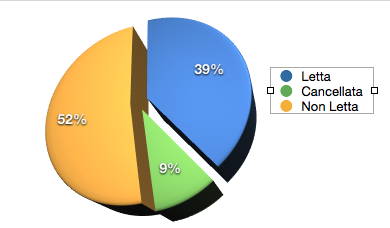
\includegraphics[scale=0.75]{img/statistica.png}
\caption{Statistica Mail}
\label{fig:statistica}
\end{figure}
Tali informazioni ci aiutano dunque a capire quanto importante e richiesto potrà essere un software di tale livello.
\newpage

\section{Descrizione generale e casi d'uso}
In questa sezione vengono presentati i casi d\textquoteright{}uso al fine di riassumere in un linguaggio intuitivo e di facile comprensione (UML2.0) ci\`{o} che il capitolato richiede. Questa non \`{e} da ritenersi un\textquoteright{}analisi completa, in quanto il prodotto se verr\`{a} sviluppato risponder\`{a} ad un numero maggiore di funzionalit\`{a} rispetto a quelle qui presentate e di questo la pianificazione ne terr\`{a} conto, in particolare dal punto di vista di costi e scadenze di consegna.

\subsection{Casi d'uso}

\subsubsection[UC0: Scenario principale]{UC0: Scenario principale}
\begin{figure}[H]
  \begin{center}
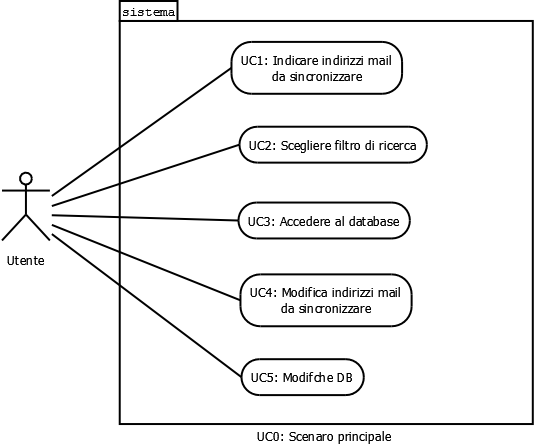
\includegraphics[width=0.60\textwidth]{img/UC0_ScenarioPrincipale.png}
\caption{UC0: Scenario principale}
\label{fig:UC0}
\end{center}
\end{figure}

\begin{description}
\item[Attori:]{utente.}
\item[Precondizione:]{il sistema visualizza la schermata iniziale dell\textquoteright{}applicativo e le infrastrutture di rete sono funzionanti.}
\item[Scenario principale:]{l\textquoteright{}utente accedendo all\textquoteright{}applicazione pu\`{o} eseguire le seguenti operazioni:
	\begin{itemize}
	\item \textbf{Indicare gli indirizzi mail da sincronizzare}: l\textquoteright{}utente pu\`{o} scegliere per quali indirizzi mail \`{e} interessato memorizzare le newsletter (UC0.1);
	\item \textbf{Scegliere filtro di ricerca}: l\textquoteright{}utente pu\`{o} scegliere dei criteri di ricerca per visualizzare i dati sul database: esso pu\`{o} visualizzare per esempio newsletter inviate presso un certo indirizzo mail, piuttosto che per data o per fornitore (UC0.2);
	\item \textbf{Accedere al database}: l\textquoteright{}utente potr\`{a} confermare il criterio di ricerca scelto e visualizzare cos\`{i} le informazioni memorizzate nel database che soddisfano la query di ricerca e quindi il sistema provveder\`{a} a visualizzare quanto chiesto dall\textquoteright{}utente (UC0.3);
	\item \textbf{Modifica indirizzi mail da sincronizzare}: l\textquoteright{}utente pu\`{o} scegliere di modificare gli indirizzi mail configurati nella sincronizzazione (UC0.4);
	\item \textbf{Modifiche DB}: l\textquoteright{}utente pu\`{o} scegliere di effettuare operazioni di modifica a parte delle informazioni memorizzate nel database(UC0.5);	
	\end{itemize}}
\item[Postcondizione per successo:]{il sistema \`{e} in attesa di una scelta da parte dell\textquoteright{}utente.}
\end{description}

\subsubsection[UC4: Modifica indirizzi mail da sincronizzare]{UC4: Modifica indirizzi mail da sincronizzare}
\begin{figure}[H]
  \begin{center}
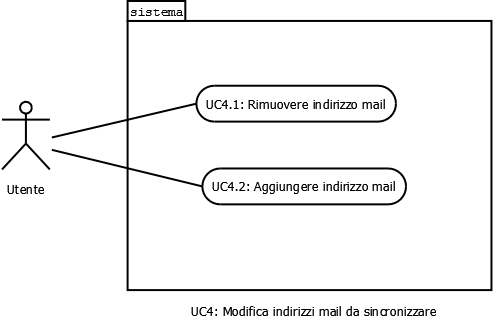
\includegraphics[width=0.60\textwidth]{img/UC4_ModificaIndirizziMailDaSincronizzare.png}
\caption{UC4: Modifica indirizzi mail da sincronizzare}
\label{fig:UC4}
\end{center}
\end{figure}

\begin{description}
\item[Attori:]{utente.}
\item[Precondizione:]{il sistema ha caricato gli indirizzi mail scelti per la configurazione e li visualizza, le infrastrutture di rete sono funzionanti.}
\item[Scenario principale:]{l\textquoteright{}utente pu\`{o} eseguire le seguenti operazioni:
	\begin{itemize}
	\item \textbf{Rimuovere indirizzi mail}: l\textquoteright{}utente pu\`{o} scegliere quali indirizzi mail rimuovere dalla sincronizzazione e quindi il sistema provveder\`{a} alla rimozione delle newsletter inviate presso quello specifico indirizzo mail (UC4.1);
	\item \textbf{Aggiungere indirizzi mail}: l\textquoteright{}utente pu\`{o} scegliere quali indirizzi mail aggiungere alla sincronizzazione (UC4.2);
	\end{itemize}}
\item[Postcondizione per successo:]{il sistema ha aggiornato gli indirizzi mail da sincronizzare.}
\end{description}

\subsubsection[UC5: Modifiche DB]{UC5: Modifiche DB}
\begin{figure}[H]
  \begin{center}
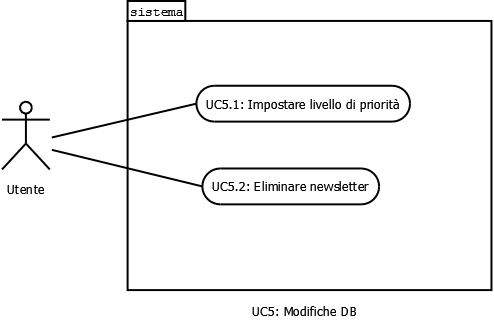
\includegraphics[width=0.60\textwidth]{img/UC5_ModificheDB.png}
\caption{UC5: Modifiche DB}
\label{fig:UC5}
\end{center}
\end{figure}

\begin{description}
\item[Attori:]{utente.}
\item[Precondizione:]{il sistema ha caricato le newsletter risultato dei filtri di ricerca scelti dall\textquoteright{}utente.}
\item[Scenario principale:]{l\textquoteright{}utente pu\`{o} eseguire le seguenti operazioni:
	\begin{itemize}
	\item \textbf{Impostare un livello di priorit\`{a}}: l\textquoteright{}utente pu\`{o} scegliere di attribuire un livello di priorit\`{a} ad una certa newsletter (UC5.1);
	\item \textbf{Rimuovere newsletter}: l\textquoteright{}utente pu\`{o} scegliere quali newsletter rimuovere (UC5.2);
	\end{itemize}}
\item[Postcondizione per successo:]{il sistema ha aggiornato le modifiche alle newsletter effettuate dall\textquoteright{}utente.}
\end{description}

\subsection{Requisiti funzionali}

\subsubsection{Obbligatori}

\begin{description}
\item[RF.ob.1:] Il software deve permettere all\textquoteright{}utente di indicare gli indirizzi mail da sincronizzare.
\item[RF.ob.2:] Il software deve permettere all\textquoteright{}utente di modificare gli indirizzi mail che ha deciso di sincronizzare.
\begin{description}
\item[RF.ob.2.1:] Il software deve permettere all\textquoteright{}utente di aggiungere un indirizzo mail per la sincronizzazione.
\item[RF.ob.2.2:] Il software deve permettere all\textquoteright{}utente di rimuovere un indirizzo mail dalla sincronizzazione.
\begin{description}
\item[RF.ob.2.2.1:] Il software deve rimuovere le newsletter ricevute all\textquoteright{}indirizzo mail eliminato dalla sincronizzazione.
\end{description}
\end{description}
\item[RF.ob.3:] Il software deve permettere all\textquoteright{}utente di selezionare la mail o le mail per le quali visualizzare le newsletter ricevute.
\begin{description}
\item[RF.ob.3.1:] Il software deve permettere all\textquoteright{}utente di visualizzare la data in cui \`{e} stata ricevuta la newsletter.
\item[RF.ob.3.2:] Il software deve permettere all\textquoteright{}utente di visualizzare il titolo delle newsletter.
\item[RF.ob.3.3:] Il software deve permettere all\textquoteright{}utente di visualizzare il contenuto delle newsletter.
\item[RF.ob.3.4:] Il software deve permettere all\textquoteright{}utente di visualizzare il fornitore del prodotto promosso nella newsletter.
\item[RF.ob.3.5:] Il software deve permettere all\textquoteright{}utente di visualizzare il contenuto del prodotto promosso nella newsletter.
\item[RF.ob.3.5:] Il software deve permettere all\textquoteright{}utente di visualizzare la fonte del prodotto promosso nella newsletter.
\item[RF.ob.3.6:] Il software deve permettere all\textquoteright{}utente di visualizzare l\textquoteright{}immagine del prodotto promosso nella newsletter.
\item[RF.ob.3.7:] Il software deve permettere all\textquoteright{}utente di modificare il database.
\begin{description}
\item[RF.ob.3.7.1:] Il software deve permettere all\textquoteright{}utente di eliminare dal database una newsletter.
\end{description}
\end{description}
\end{description}

\subsubsection{Desiderabili}

\begin{description}
\item[RF.de.1:] Il software deve permettere all\textquoteright{}utente di assegnare una priorit\`{a} alle newsletter.
\begin{description}
\item[RF.de.1.1:] Il software deve permettere all\textquoteright{}utente di assegnare dei valori di priorit\`{a} da 1 a 5.
\begin{description}
\item[RF.de.1.1.1:] Un valore di priorit\`{a} pari a 1 dovr\`{a} indicare un valore di scarsissima priorit\`{a}.
\item[RF.de.1.1.2:] Un valore di priorit\`{a} pari a 2 dovr\`{a} indicare un valore di bassa priorit\`{a}.
\item[RF.de.1.1.3:] Un valore di priorit\`{a} pari a 3 dovr\`{a} indicare un valore di normale priorit\`{a}.
\item[RF.de.1.1.4:] Un valore di priorit\`{a} pari a 4 dovr\`{a} indicare un valore di media priorit\`{a}.
\item[RF.de.1.1.5:] Un valore di priorit\`{a} pari a 5 dovr\`{a} indicare un valore di alta priorit\`{a}.
\end{description}
\end{description}
\item[RF.de.2:] Il software deve permettere di effettuare delle visualizzazioni di newsletter filtrando in base a criteri di ricerca scelti dall\textquoteright{}utente.
\begin{description}
\item[RF.de.2.1:] Il software deve permettere di filtrare le newsletter per indirizzi mail.
\item[RF.de.2.2:] Il software deve permettere di filtrare le newsletter per data.
\item[RF.de.2.3:] Il software deve permettere di filtrare le newsletter per priorit\`{a}.
\item[RF.de.2.4:] Il software deve permettere di filtrare le newsletter per fonte.
\item[RF.de.2.5:] Il software deve permettere di filtrare le newsletter per fornitore.
\end{description}
\end{description}
 

\newpage

\section{Analisi di fattibilità}
\subsection{Aspetto marketing}
\subsection{Target}
Il segmento di mercato al quale \NOMEPROGETTO{} si rivolge è costituito dalla nicchia di mercato rappresentata da un utenza business, la quale ha la necessità di catalogare con precisione e senza perdite di tempo, le numerose newsletter che quotidianamente giungono alla casella di posta elettronica.\\
Nello specifico si vogliono raggiungere i \emph{liberi professionisti} quali avvocati, architetti, ingegneri, ma anche \emph{imprenditori} di PMI che spesso gestiscono personalmente un account di posta.\\
Tutti questi soggetti hanno la necessità di gestire con efficienza le email ma spesso non hanno il tempo necessario per farlo in modo efficace: \NOMEPROGETTO{} riesce a colmare esattamente questa lacuna rendendo ogni operazione intuitiva ed immediata.

\subsection{Competitors}
Per approfondire la conoscenza del mercato dei software di gestione delle email si è resa necessaria una ricerca approfondita dei possibili competitors presenti nel panorama internazionale, in modo da comprendere al meglio i pregi e i difetti di tali soluzioni per poter implementare caratteristiche innovative e peculiarità uniche tali da rendere \NOMEPROGETTO{} un prodotto unico nel suo genere.

\subsubsection{G-lock Email Processor} 
\url{http://www.glocksoft.com/email-processor}

\begin{figure}[H]
\centering
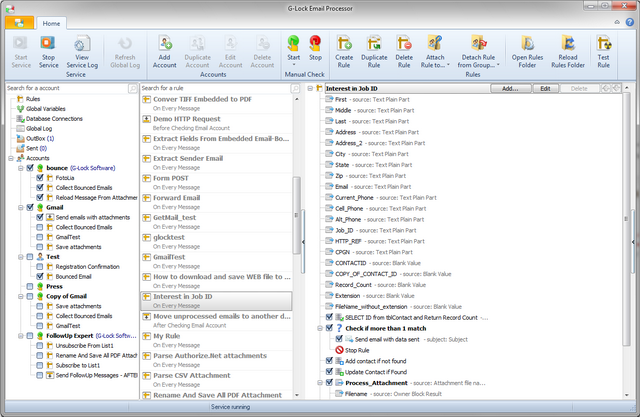
\includegraphics[scale=0.5]{img/gep-main-window-1.png}
\caption{Schermata G-Lock Email Processor}
\end{figure}

Il software è in grado di:
\begin{itemize}
\item Controllare automaticamente l'account di posta in modo regolare ed elaborare i messaggi in background;
\item Convertire il contenuto del messaggio in record di database;
\item Salvare i dati estratti dal messaggio in un file;
\item Salvare gli allegati dei messaggi sul disco;
\item Creare un report in formato PDF o HTML;
\item Integrare i dati estratti in Microsoft Outlook;
\item Ottimizzare il proprio business ed il servizio al cliente con l'invio di risposte automatiche;
\item Convertire automaticamente i dati estratti utilizzando MS Windows script;
\item Estrarre URL da e-mail e processare dati da pagine web e feed RSS;
\end{itemize}

\begin{figure}[H]
\centering 
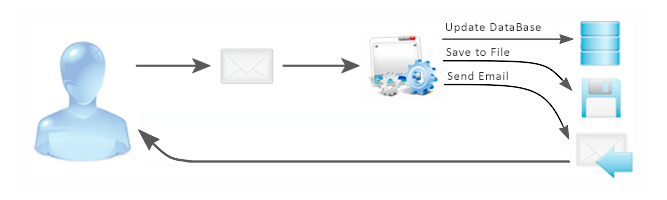
\includegraphics[scale=2]{img/emailprocessor.png} 
\caption{Funzionalità G-Lock Email Processor}
\end{figure}

Il software si presenta come la migliore soluzione trovata sul mercato ma possiede alcuni importanti difetti: è compatibile solamente per la piattaforma Microsoft Windows, il quale ricopre un'ampia fetta di mercato ma non la totalità, e il prezzo è considerevolmente alto per una singola licenza, 295 USD.
\newpage

\subsubsection{Email2db}
\url{http://www.email2db.com/email-to-database.aspx}

\begin{figure}[H]
\centering 
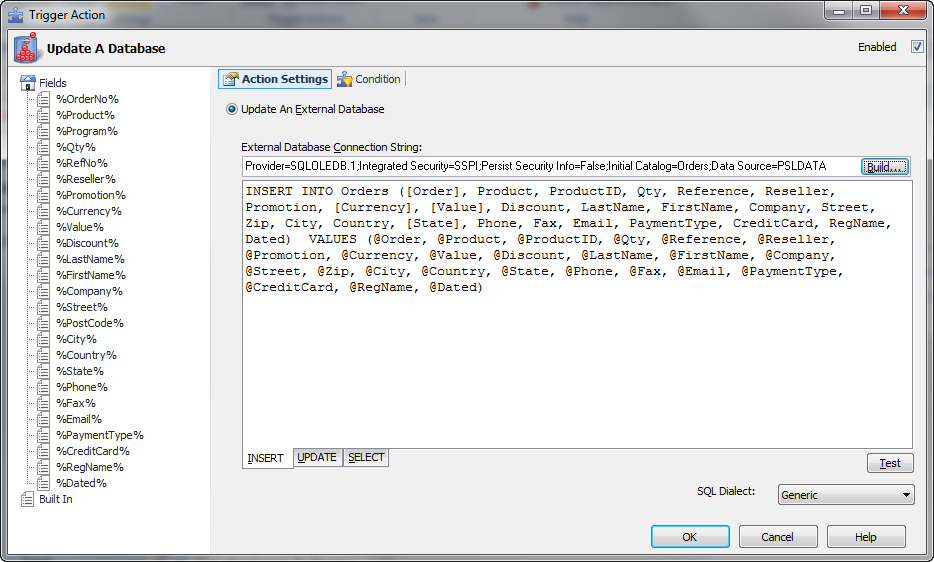
\includegraphics[scale=0.6]{img/email2db.png} 
\caption{Schermata Trigger Email2db}
\end{figure}

Email2DB è uno strumento per l'automazione di messaggi che è possibile utilizzare per convertire email e altri tipi di messaggi in record per database ed inoltre permette di convertire qualsiasi forma di messaggio anche in formato Excel o in record CSV.

Il software è grado di:
\begin{itemize}
\item i leggere messaggi e-mail provenienti da più fonti (server POP3, server IMAP, server Exchange, feed di Twitter, pagine Web, feed RSS e database esterni);
\item creare un numero qualsiasi di trigger. Il trigger è un insieme di condizioni che Email2DB verifica (per esempio, uno specifico mittente o parole specifiche nell'oggetto). Se un messaggio supera le condizioni del trigger, Email2DB elabora una serie di azioni su di esso. Queste azioni comprendono l'aggiornamento di una banca dati, l'invio di eventuali risposte e-mail e report di stampa;
\item analizzare ed estrarre dati da e-mail e aggiornare diversi tipi di database, tra cui SQL Server, MySQL, Oracle, Pervasive, Access e qualsiasi altro database che supporti ADO o ODBC;
\item salvare i dati su foglio di calcolo Excel o file CSV.
\end{itemize}

Email2DB è disponibile in diverse versioni: Small Business, Enterprise, Data Center \& Developer.\\
Tutte le edizioni includono le stesse funzionalità per l'analisi e l'estrazione di dati da e-mail per aggiornare più database, permettono di gestire un numero illimitato di account e trigger per l'elaborazione.\\
Inoltre tutte le edizioni non hanno restrizioni sul tipo di messaggi che possono analizzare (Server POP3, IMAP, feed di Twitter) ma per esempio solo le versioni Enterprise e Developer permettono di spostare il messaggio corrente in una cartella diversa da quella in cui è arrivato.

Anche per questo software sorge lo stesso problema del precedente in quando è utilizzabile solo su piattaforme Windows 7/8, Vista, XP, 2003 Server, 2008 Server, 2012 Server.\\
Il software è a pagamento con un costo a partire da 475\euro per l'edizione Small Business, 995\euro per quella Enterprise, 475\euro per quella Developer e 3195\euro per la Data Center Edition, ma permette una prova gratuita di 30 giorni dopo essersi registrati.

\subsection{Valore aggiunto}
Dall'analisi dei competitors è emerso come non esista sul mercato un software \emph{multipiattaforma} che soddisfi i bisogni riscontrati nel capitolato; questa è una notevole mancanza in quanto non esiste solo il mondo Microsoft, anzi il mercato dei sistemi operativi sta andando incontro a notevoli cambiamenti, soprattutto con l'avvento dei terminali mobile e di Android; risulta evidente come non basta più coprire la fetta maggiore di pubblico, ma è necessario rendere il prodotto fruibile alla maggior parte delle persone e dei dispositivi.

\subsection{Aspetto tecnologico}
Il progetto consta nella realizzazione di un software per computer desktop in grado di essere utilizzabile su diversi sistemi operativi tra i quali \emph{Microsoft Windows}, \emph{Apple Mac OSX} e \emph{GNU}\textbackslash\emph{Linux}.\\
Per ottenere tale risultato si è scelto di utilizzare \emph{Java}\footnote{\url{http://it.wikipedia.org/wiki/Java\_\%28linguaggio\_di\_programmazione\%29}}, un linguaggio di programmazione multipiattaforma semi-interpretato che consente di scrivere programmi che vengono eseguiti su di una macchina virtuale installabile sui tutti i sistemi operativi sopracitati.\\
Il progetto, per rispondere ai requisiti, deve risolvere 3 problematiche principali che sono a loro volta legate a 3 differenti tecnologie informatiche:
\begin{itemize}
\item \textbf{Accesso ai server di posta:} per recuperare le email contenti le newsletter di interesse, si deve poter accedere ai server di posta che le contengono; esistono innumerevoli provider che forniscono tale servizio agli utenti, sia per uso personale e gratuiti, che per uso professionale e a pagamento.\\
Per non porre limiti nell'utilizzo del software di dovrà quindi sviluppare un sistema che sia in grado di connettersi indipendentemente a qualsiasi server di posta: per ottenere questo risultato si dovrà utilizzare la \emph{JavaMail API}\footnote{\url{http://docs.oracle.com/javaee/7/api/}} presente  nella \emph{Java Enterprise Edition}.
\item \textbf{Lettura della newsletter:} le email strutturate, come possono essere le newsletter, sono composte mediante il linguaggio di markup \emph{HTML}; questo consente di leggere molto facilmente il contenuto dei messaggi ma pone un problema da non sottovalutare: infatti tale linguaggio, pur essendo standard, non fornisce un modo universale di strutturare le informazioni, ma lascia al programmatore ampia libertà di scrittura.\\
Con alta probabilità ogni newsletter proveniente da un'azienda avrà una struttura molto diversa da quella proveniente da una seconda azienda; per questo motivo si è deciso di personalizzare il prodotto in base alle esigenze di ogni singolo cliente.\\
Lo strumento che consentirà di analizzare in modo efficiente le diverse tipologie di newsletter è la libreria \emph{Jsoup}\footnote{\url{http://jsoup.org/}}. Libreria open source scritta in Java e quindi facilmente utilizzabile all'interno del progetto.
\item \textbf{Salvataggio delle informazioni nel database:} dopo aver ottenuto le informazioni da una newsletter si presenta la necessità di conservarle in modo persistente nella memoria di massa del personal computer del cliente.\\
Il modo migliore di salvare tali informazioni è quello di utilizzare un database dal quale si potranno, in un secondo momento, recuperare tutte le notizie volute impostando ricerche specifiche a discrezione dell'utente.\\
Per realizzare la base di dati si è scelto \emph{Oracle MySQL}\footnote{\url{http://it.wikipedia.org/wiki/MySQL}}, DBMS open source disponibile per i 3 sistemi operativi di riferimento, in quanto sono disponibili driver JDBC che consentono un'agevole gestione delle connessioni al database e delle relative query.
\end{itemize}

\subsection{Aspetto legale}
Il prodotto in questione come emerso dall\textquoteright{}analisi dei competitor non è una novità, quindi le strategie che verranno adottate sono basate sia sull'aggiunta di caratteristiche qualitative al prodotto sia strategie di pricing dato che lo sviluppo del prodotto non utilizzerà nuove tecnologie, ma tecnologie già conosciute. \\
La legge disciplina specificatamente la tutela del software, in primo luogo con la legge sul diritto d'autore, a seguito del Decreto Legislativo 29 Dicembre 1992 n. 518. In secondo luogo, la legge sul diritto d'autore protegge il codice sorgente del software ed il relativo codice oggetto. La tutela è estesa al lavoro di progettazione architetturale e successivamente di dettaglio per la definizione costruttiva del software.\\
La tutela si estende anche all'interfaccia del programma stesso. Ma, se quest'ultima contiene particolari immagini da proteggere, ciò andrà fatto indipendentemente, in base ad altre norme. Tuttavia la tutela del diritto d'autore non è l'unica forma di protezione da considerare per vedere tutelate le soluzioni tecniche trovate per realizzare un software. Analizziamo dunque altre forme quali: il brevetto, il marchio, la protezione del design, e più approfonditamente il diritto d'autore.

\subsubsection{Il brevetto (software)}
<<<<<<< HEAD
Per definizione un brevetto \textit{``è lo strumento giuridico che permette di commercializzare in esclusiva la propria invenzione in un certo territorio''}. E nello specifico, con brevetto software ci si riferisce, secondo la definizione adottata dall'Unione Europea, ad un brevetto applicato ad \textit{``una invenzione realizzata per mezzo di un elaboratore''}. La legislazione in materia è regolata dalla Convenzione europea dei Brevetti, degli anni '70. L'interpretazione lascia presupporre che, nel caso di invenzioni implementate con l'utilizzo di un calcolatore, per ottemperare ai requisiti di brevettabilità vi deve per forza essere una soluzione tecnica adeguata a risolvere un problema tecnico in modo nuovo ed inventivo rispetto allo Stato dell'Arte, che va oltre la normale interazione tra software e hardware.\\
Il prodotto software che il team di progetto intende sviluppare non sarà brevettabile secondo la vigente normativa europea, poiché non realizzerà una nuova soluzione tecnica per risolvere in maniera inventiva almeno un problema tecnico, dato che offrirà fondamentalmente la consultazione di una knowledge base, specificatamente creata e gestibile, a fini commerciali.\\
Anche l'aspetto delle eventuali violazioni del diritto di privativa (diritto al monopolio) detenuto da terzi è da escludersi a priori, visto che da un'analisi normativa si è accertata l'impossibilità di brevettare la nostra tipologia di software, e quindi che nessun'altra realtà applicativa simile alla nostra abbia potuto acquisire nel passato un brevetto quale garanzia di privativa.
=======
Per definizione un brevetto \textit{``è lo strumento giuridico che permette di commercializzare in esclusiva della propria invenzione in un certo territorio''}. E nello specifico, con brevetto software ci si riferisce, secondo la definizione adottata dall'Unione Europea, ad un brevetto applicato ad \textit{``una invenzione realizzata per mezzo di un elaboratore''}. La legislazione in materia è regolata dalla Convenzione europea dei Brevetti, degli anni '70. L'interpretazione lascia presuppore che, nel caso di invenzioni implementate con l'utilizzo di un calcolatore, per ottemperare ai requisiti di brevettabilità vi deve per forza essere una soluzione tecnica adeguata a risolvere un problema tecnico in modo nuovo ed inventivo rispetto allo Stato dell'Arte, che va oltre la normale interazione tra software e hardware.\\
Il prodotto software che il team di progetto intende sviluppare non sarà brevettabile secondo la vigente normativa europea, poiché non realizzerà una nuova soluzione tecnica per risolvere in maniera inventiva almeno un problema tecnico, dato che questa è già stata brevettata. Il team dovrà quindi provvedere a ottenere una licenza per vendere il prodotto in un mercato internazionale. \\
>>>>>>> b43c12d1f545e02658eb5209325481d34dda08e1

\subsubsection{Il brevetto (hardware)}
La situazione per la parte hardware del progetto è simile alla parte software.\\
Nessuna normativa nazionale o europea ci dà facoltà di brevettare la struttura da noi realizzata per il nostro progetto, in quanto non dispone a tutti gli effetti di una tecnologia particolare per la realizzazione, ma è costituita da risorse intellettuali e/o fisiche già coperte da brevetto.\\
<<<<<<< HEAD
Possiamo quindi giungere alla conclusione che dal punto di vista brevettuale non siamo in grado di tutelarci in modo adeguato da un eventuale concorrente nel settore.
=======
Dal punto di vista brevettuale quindi non possiamo che fare un apposito contratto con l'azienda direttamente interessata NRI \& NCC (istituto di ricerca giapponese). La ricerca è stata effettuata presso la banca dati dell'EPO digitando la keyword \textit{``newsletter''}, 
\url{http://worldwide.espacenet.com/publicationDetails/biblio?DB=EPODOC\&II=9\&ND=3\&adjacent=true\&locale=en\_EP\&FT=D\&date=20040527\&CC=JP\&NR=2004152051A\&KC=A}.
>>>>>>> b43c12d1f545e02658eb5209325481d34dda08e1

\subsubsection{Il marchio}
La nostra esperienza ha mostrato che la registrazione di un marchio, cioè una parola o un simbolo da utilizzare in esclusiva per identificare un prodotto (software nel nostro caso), vietando ad altri di poter utilizzare quello stesso simbolo, è molto conveniente, per i bassi costi, e per gli straordinari vantaggi pratici ed economici che se ne ricavano. Il nuovo marchio dura dieci anni dalla data di deposito, ma rinnovabili alla scadenza. Per ogni marchio che il team vorrà registrare verrà adottatate la seguente scelte:
\begin{itemize}
\item registrazione di un marchio verbale, cioè formato solamente da parole, così da godere del diritto esclusivo di utilizzare il marchio con qualsiasi grafica;
\item registrazione di un marchio dal segno ``in bianco/nero'', così da tutelare per tutti i colori o loro combinazioni da attribuire al nostro marchio;
\item indicazione dell'appartenenza del marchio alla classe di servizi (n. 42) ``Servizi nell'ambito della scienza e della tecnologia, come servizi di ricerca e di sviluppo relativi a ciò, analisi e ricerche industriali, progettazione e sviluppo di computer, consulenza e assistenza legale.''
\item registrazione di un marchio internazionale, (valido nei Paesi che hanno aderito agli inerenti accordi internazionali), piuttosto che nazionale ovvero valido solo nel nostro Paese, o  comunitario (efficace nei Paesi appartenenti all'Unione Europea). Questa scelta è stata dettata dal fatto che il servizio che forniremo attraverso un'applicazione web potrebbe trovare concorrenza e quindi necessitare di tutela in ambito internazionale, visto anche che verrà rilasciato in più lingue, dunque sarebbe un errore non stendere la protezione territoriale mediante un marchio internazionale.
I marchi che il team dovrà provvedere a registrare sono: \textit{Malla5} e \textit{Mail2you}. Le somme previste per ogni marchio, comprensive di tasse, onorari e tutela dei diritti per 10 anni sono pari a 2000\officialeuro.
\end{itemize}

\subsubsection{Design}
Si può proteggere l'aspetto esteriore di un prodotto, l'interfaccia grafica del software in questo caso, registrandone il design. Per essere registrabile è sufficiente che abbia un carattere individuale, ossia che per le sue caratteristiche si differenzi da tutti gli altri; ma questo potrebbe risultare (sarà una scelta di progettazione) vero soltanto in parte, dato anche che l'applicazione avrà un layout generico e non particolareggiante. Pertanto, anche supponendo di realizzare il design con elementi grafici particolari, riteniamo che la spesa per tale registrazione (circa 850 Euro), sia troppo onerosa e sostanzialmente superflua da sostenere.

\subsubsection{Il diritto d'autore}
<<<<<<< HEAD
La legislazione sul diritto d'autore (disciplinato prevalentemente dalla Legge 22 aprile 1941, n. 633, e dalla Convenzione di Berna), figura propria degli ordinamenti di \textit{civil law}, tra i quali troviamo l'Italia, mentre in quelli di \textit{common law} esiste l'istituto del copyright, permette di tutelare dal plagio molte tipologie di opere creative, tra le quali il software per computer. La legge protegge la forma di realizzazione del servizio o dell'opera, e non l'idea che vi era alla base. Nel nostro caso consideriamo che saremo titolari dei diritti (patrimoniali e morali) sull'opera. Per quanto concerne l'acquisto del diritto d'autore, esso si acquista ``automaticamente'' per il solo fatto della creazione dell'opera, senza oneri di carattere amministrativo.\\
Ciononostante, per dare all'impresa una prova certa della paternità dell'opera, si rende necessario il deposito dell'opera agli uffici predisposti. Va aggiunto che il deposito alla SIAE (Società Italiana degli Autori ed Editori) è talvolta necessario per l'esercizio dei diritti connessi. In Italia, il deposito dell'opera si divide in: deposito di opera inedita, da effettuare alla SIAE prima della pubblicazione dell'opera, e deposito di opera pubblicata, da effettuare ancora presso la SIAE (Sezione OLAF, che cura la tenuta di un apposito Registro pubblico). Si nominano in coda i diritti che l'autore acquista sulla propria opera: il diritto esclusivo di riproduzione, di esecuzione, di diffusione, di distribuzione, di noleggio, di prestito, di elaborazione e trasformazione; diritti cedibili dietro compenso.
=======
La legislazione sul diritto d'autore (disciplinato prevalentemente dalla Legge 22 aprile 1941, n. 633, e dalla Convenzione di Berna), figura propria degli ordinamenti di civil law, tra i quali l'Italia, invece in quelli di common law c'è l'istituto del copyright, permette di tutelare dal plagio molte tipologie di opere creative, tra le quali il software per computer. La legge protegge la forma di realizzazione del servizio o dell'opera, e non l'idea che vi era alla base. Nel nostro caso consideriamo che saremo titolari dei diritti (patrimoniali e morali) sull'opera. Per quanto concerne l'acquisto del diritto d'autore, esso si acquista ``automaticamente'' per il solo fatto della creazione dell'opera, senza oneri di carattere amministrativo.\\
Ciononostante, per dare all'impresa una prova certa della paternità dell'opera, si rende necessario il deposito dell'opera agli uffici predisposti. Va aggiunto che il deposito alla SIAE (Società Italiana degli Autori ed Editori) è talvolta necessario per l'esercizio dei diritti connessi. In Italia, il deposito dell'opera si divide in: deposito di opera inedita, da effettuare alla SIAE prima della pubblicazione dell'opera, e deposito di opera pubblicata, da effettuare ancora presso la SIAE (Sezione OLAF, che cura la tenuta di un apposito Registro pubblico). Si nominano in coda i diritti che l'autore acquista sulla propria opera: il diritto esclusivo di riproduzione, di esecuzione, di diffusione, di distribuzione, di noleggio, di prestito, di elaborazione e trasformazione; diritti cedibili dietro compenso. Le tariffe per il deposito del nostro prodotto, inteso come opera inedita, presso la SIAE è stimata in una quota annuale di 261,81\officialeuro.
>>>>>>> b43c12d1f545e02658eb5209325481d34dda08e1

\subsubsection{Trattamento dei dati}
%TODO


\subsection{Aspetto economico-finanziario}
\newpage

\section{Pianificazione}
\subsection{Work Breakdown Structure}
La Work BreakDown Structure, d'ora in poi WBS, rappresenta l'insieme delle attivit\`{a} necessarie a svolgere un compito ben preciso o un processo. Le singole attivit\`{a} prendono il nome di Work Package, WP, e definiscono dettagliatamente le azioni da svolgere per
ciascuna di esse.\\
La WBS \`{e} costituita da una struttura ad albero di WP che, a partire dell'obiettivo finale del progetto, specifica per suddivisioni successive i singoli sotto-obiettivi, fino all'unit\`{a} minima di attivit\`{a}.\\
Tale scomposizione in tanti compiti di dimensioni limitate facilita la gestione, il controllo e l'assegnazione delle singole attivit\`{a}, consentendo una migliore suddivisione del lavoro.\\
Grazie alla WBS il project manager pu\`{o}, in maniera semplificata, organizzare tutte le attivit\`{a} che compongono il progetto, cos\`{i} come i WP, ed avere sempre a disposizione un utile strumento che definisce tutti i passi necessari alla buona realizzazione del progetto.\\
La WBS, inoltre, risulta essere la base per tutte le altre attivit\`{a} di pianificazione richieste per la realizzazione di un progetto di successo.

\begin{figure}[H]
\centering % per centrare l'immagine (opzionale)
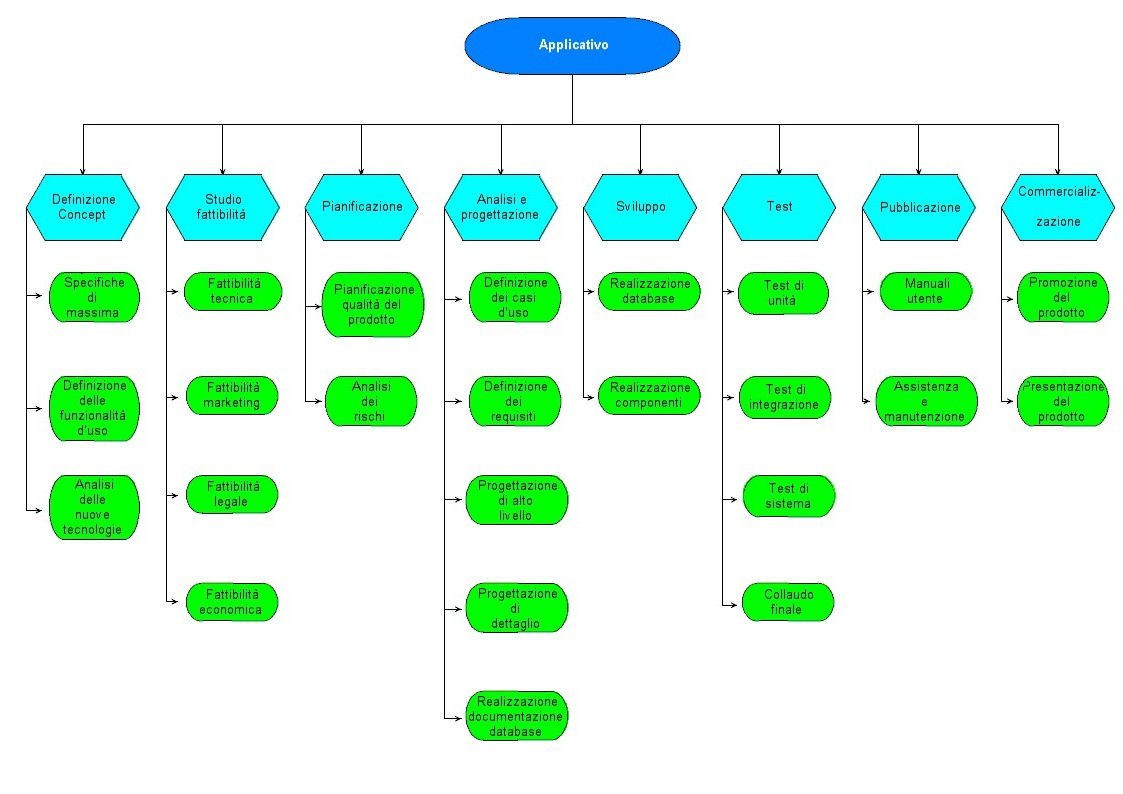
\includegraphics[scale=0.5]{img/Progetto.jpg}
\caption{Diagramma WBS}
\label{fig:Diagramma WBS}
\end{figure}

\subsubsection{WBS-Primo Livello}
\paragraph{Definizione Concept (1.1)}
\`{e} la prima fase del progetto, dove si raccolgono le idee per portare alla nascita e alla definizione del progetto.\\
A partire da questo momento in poi si penser\`{a} alla forma che assumer\`{a} il prodotto finale, alla  definizione delle caratteristiche pi\`{u} importanti (target del prodotto, come si intende erogare il servizio) e alla definizione delle funzionalit\`{a} principali che il prodotto finale deve avere.

\paragraph{Studio Fattibilit\`{a} (1.2)}
\`{e} la fase successiva a quella di Definizione Concept, ha lo scopo di capire se quello che si vuole realizzare \`{e} innanzitutto fattibile e possa portare ad avere dei guadagni concreti.\\
Dunque il concept viene valutato sotto tutti i punti di vista e di interesse per l'organizzazione, al fine di avere un insieme di conclusioni e indicazioni sulle possibilit\`{a} di buona riuscita del lavoro.

\paragraph{Pianificazione (1.3)}
In questa fase si vogliono studiare i processi che il team vuole adottare, quindi una pianificazione delle attivit\`{a} inerenti il ciclo di vita del prodotto avvalendosi di strumenti come diagrammi di Gantt, WBS, OBS e altri strumenti consultabili alla sezione Pianificazione. In questa fase si vogliono definire anche gli obiettivi e le strategie al fine di stabilire a priori ci\`{o} che il team dovr\`{a} controllare e soprattutto misurare.

\paragraph{Analisi e Progettazione (1.4)}
A questo punto gli obiettivi del progetto sono chiari, bisogna dunque formalizzarli e chiarirli in maniera non ambigua.\\
Vengono illustrate dettagliatamente le funzionalit\`{a}, i servizi e le prestazioni che dovranno essere offerte dal prodotto finito.\\
Infine viene progettato come il prodotto soddisfer\`{a} i requisiti definiti in precedenza, definendone la struttura ed architettura da assumere e rispettare.

\paragraph{Sviluppo (1.5)}
In questa fase si passa alla creazione vera e propria del prodotto software mediante la codifica di quanto definito durante la progettazione.\\
Affinché questo risulti possibile \`{e} essenziale che ogni membro si attenga strettamente a quanto descritto nei documenti che gli vengono forniti.\\
Non deve, assolutamente, inserire della creativit\`{a} personale, in quanto il suo compito consiste nella traduzione in codice di quanto deciso precedentemente.\\
Il codice prodotto dovr\`{a} essere costantemente verificato, per avere la sicurezza e la certezza che rispetti i requisiti di qualit\`{a} definiti nella fase di pianificazione, accompagnato dall'appropriata manualistica.

\paragraph{Test (1.6)}
Arrivati a questo punto vengono dunque effettuati i test delle componenti prodotte, verificando come si relazionano tra di loro, a partire dalle componenti di base del prodotto per arrivare a testare, alla fine, il sistema completo.\\
Inoltre viene verificato che quanto \`{e} stato prodotto sia conforme agli obiettivi e ai requisiti che si erano definiti in precedenza.

\paragraph{Post vendita (1.7)}
Una volta che il software prodotto \`{e} terminato e rispetta gli obiettivi ed i requisiti, viene avviato il piano per il rilascio.\\
In questa fase \`{e} prevista la realizzazione di documentazione a supporto dell'utente finale ed eventuali attivit\`{a} di manutenzione o comunque di supporto all'utente finale.\\

\paragraph{Commercializzazione (1.8)}
Questa fase \`{e} stata pianificata al fine di definire come la societ\`{a} intende promuovere il proprio prodotto, ricercare eventuali partnership.

\subsubsection {WBS-Secondo livello}
Per la descrizione dei Work Package di secondo livello verr\`{a} utilizzato il seguente schema in quanto,
, rappresentano tutti insiemi di attivit\`{a} elementari da realizzare:
\begin{description}
\item[Descrizione:] descrizione generica su ci\`{o} che il WP si propone di fare.
\item[Responsabile:] persona che ha la responsabilit\`{a} delle attivit\`{a} da svolgere nel WP e dell'output finale.
\item[Input:] Ci\`{o} di cui necessita in ingresso il WP per iniziare a svolgere le sue attivit\`{a}. Solitamente questi input vengono forniti in uscita da altri WP e possono essere prototipi, documenti o risorse.
\item[Output:] ci\`{o} che il WP deve produrre in uscita. I tipi di uscita possono essere diversi, a seconda delle attivit\`{a} svolte.
\item[Attivit\`{a}:] lista delle attivit\`{a} elementari necessarie al completamento del WP. Per poter essere considerato concluso un WP devono essere concluse tutte le sue attivit\`{a}.
\item[Costo:] costo in euro riassuntivo di tutte le spese necessarie al compimento del WP. Andranno considerate le spese relative al consumo di tutte le risorse utilizzate.
\item[Tempi di realizzazione:] tempo necessario stimato per la buona riuscita e per il completamento del WP, espresso in giorni lavorativi.
\end{description}

\paragraph{Specifiche di massima (1.1.1)}
\begin{description}
\item[Descrizione:] Definizione delle prime specifiche del prodotto per individuare i requisiti ad alto livello necessari a sviluppare l'abstract.
\item[Responsabile:]
\item[Input:] idee, critiche e specifiche provenienti da un brainstorming di gruppo.
\item[Output:] documento formale che descrive una prima versione della specifica del prodotto, nella quale si definisce dettagliatamente l'idea che si vuole realizzare.
\item[Attività:]\mbox{}\\[-1.5\baselineskip]
	\begin{itemize}
	\item ricerca nel web di eventuali competitors per ricavare da progetti gi\`{a} esistenti quali funzionalit\`{a} \`{e} bene riproporre, quali no e quali sono quelle innovative che bisogna sviluppare;
	\item brainstorming tra le risorse umane assegnate al WP per identificare caratteristiche da implementare nel prodotto;
	\item prima stesura documento;
	\item verifica documento ed eventuali correzioni;
	\item formalizzazione documento;
	\item approvazione;
	\end{itemize}
\item[Costo:] 270 \euro{}

\paragraph{Definizione delle funzionalit\`{a} d'uso (1.1.2)}
\begin{description}
\item[Descrizione:] definizione dettagliata delle pi\`{u} importanti funzionalit\`{a} che si vuole siano presenti all'interno del software.
\item[Responsabile:]
\item[Input:] documento di specifiche di massima prodotto dal WP.
\item[Output:] documento che descrive nel dettaglio le funzionalità base che si è deciso di sviluppare.
\item[Attività:]\mbox{}\\[-1.5\baselineskip]
	\begin{itemize}
	\item studio del documento prodotto dal WP;
	\item analisi tecnica di sistemi simili gi\`{a} esistenti;
	\item prima stesura del documento;
	\item verifica del documento ed eventuali correzioni;
	\item formalizzazione del documento;
	\item approvazione.
	\end{itemize}
\item[Costo:] 385 \euro{}
\item[Tempi di realizzazione:] 4 giorni lavorativi.
\end{description}

\paragraph{Analisi delle nuove tecnologie (1.1.3)}
\begin{description}
\item[Descrizione:] ricerca mirata di eventuali innovazioni tecnologie presenti nel mercato che possano risultare utili allo sviluppo del software.
\item[Responsabile:]
\item[Input:] documento di specifiche di funzionalit\`{a} prodotto dal WP.
\item[Output:] documento che descrive nel dettaglio eventuali nuove tecnologie interessanti che potrebbero essere inserite nel progetto. Per ciascuna di queste viene riportata una stima di tempo che si presuppone sia necessario ai programmatori per arrivare ad averne una buona padronanza.
\item[Attività:]\mbox{}\\[-1.5\baselineskip]
	\begin{itemize}
	\item studio del documento prodotto dal WP;
	\item analisi mirata di eventuali nuove tecnologie e stima delle ore per l'apprendimento;
	\item prima stesura documento;
	\item verifica documento ed eventuali correzioni;
	\item formalizzazione documento;
	\item approvazione.
	\end{itemize}
\item[Costo:] 279 \euro{}
\item[Tempi di realizzazione:] 3 giorni lavorativi.
\end{description}

\paragraph{Fattibilit\`{a} tecnica (1.2.1)}
\begin{description}
\item[Descrizione:] fase di valutazione del prodotto che si vuole realizzare dal punto di vista tecnico-tecnologico.
\item[Responsabile:] 
\item[Input:] tutti i documenti prodotti dal secondo livello del WP.
\item[Output:] documento che descrive nel dettaglio, in modo non ambiguo, la fattibilità tecnica per il prodotto che si vuole realizzare indicando le tecnologie e gli strumenti necessari per farlo.
\item[Attività:]\mbox{}\\[-1.5\baselineskip]
	\begin{itemize}
	\item studio dei documenti prodotti dai WP;
	\item incontro fra responsabili i tecnici;
	\item valutazione dei sistemi e degli standard in uso;
	\item valutazione delle tecnologie;
	\item prima stesura documento riassuntivo;
	\item verifica documento ed eventuali correzioni;
	\item formalizzazione documento;
	\item approvazione;
	\end{itemize}
\item[Costo:] 335 \euro{}
\item[Tempi di realizzazione:] 3 giorni lavorativi.
\end{description}

\paragraph{Fattibilit\`{a} marketing (1.2.2)}
\begin{description}
\item[Descrizione:] fase di analisi del mercato per studiare la concorrenza dovuta ad idee similari. Seguono quindi una stima ed una analisi della redditivit\`{a} del prodotto e alle indicazioni preliminari su come pubblicizzarlo e rilasciarlo al fine di ottenere maggiori introiti dalla vendita.
\item[Responsabile:] 
\item[Input:] ricerche di mercato e dati riguardanti eventuali competitor.
\item[Output:] documento formale che indica la fattibilità dal punto di vista del marketing. Nel caso di una buona riuscita sono riportate anche le azioni da seguire per il rilascio del prodotto.
\item[Attività:]\mbox{}\\[-1.5\baselineskip]
	\begin{itemize}
	\item analisi di mercato;
	\item interviste, sondaggi e dialoghi con possibili clienti;
	\item individuazione di eventuali strategie;
	\item prima stesura documento riassuntivo;
	\item verifica documento ed eventuali correzioni;
	\item formalizzazione documento;
	\item approvazione;
	\end{itemize}

\item[Costo:] 319 \euro{}
\item[Tempi di realizzazione:] 3 giorni lavorativi.
\end{description}
\paragraph{Fattibilit\`{a} legale (1.2.3)}
\begin{description}
\item[Descrizione:] fase di analisi del prodotto software sotto l'aspetto legale. Si studiano e si definiscono le strategie eventuali da adottare in difesa del progetto. Si verifica inoltre la possibilit\`{a} di brevettare il prodotto e di registrare un marchio. Infine si verifica che lo sviluppo non porti alla violazione di alcuna legge o normativa in vigore.
\item[Responsabile:]
\item[Input:] conoscenza di eventuali prodotti simili nel mercato e normative/vincoli legali.
\item[Output:] documento formale che indica la fattibilità dal punto di vista legale. Se viene prevista una buona riuscita allora sono riportate anche le azioni da seguire per il corretto rilascio del prodotto.
\item[Attività:]\mbox{}\\[-1.5\baselineskip]
	\begin{itemize}
	\item definizione di un marchio;
	\item consulenza esterna legale;
	\item prima stesura documento riassuntivo;
	\item verifica documento ed eventuali correzioni;
	\item formalizzazione documento;
	\item approvazione;
	\end{itemize}

\item[Costo:] 315 \euro{}
\item[Tempi di realizzazione:] 3 giorni lavorativi.
\end{description}
\paragraph{Fattibilit\`{a} Economica (1.2.4)}
\begin{description}
\item[Descrizione:] fase di analisi del prodotto software sotto l'aspetto economico. Si studia e si valutano i benefici economici che tale progetto potrebbe portare. Vengono stimati inoltre i costi che l'organizzazione dovrebbe sostenere, diretti ed indiretti. Inoltre viene studiata la possibilit\`{a} di ottenere dei finanziamenti esterni 
\item[Responsabile:] 
\item[Input:] conoscenza dei costi diretti ed indiretti delle varie risorse.
\item[Output:] documento formale che indica la fattibilità dal punto di vista economico. All'interno di questo verrà illustrata la previsione economica del prodotto, illustrando i possibili guadagni ed indicando l'eventuale punto di pareggio.
\item[Attività:]\mbox{}\\[-1.5\baselineskip]
	\begin{itemize}
	\item consulenze economiche;
	\item stima dei costi, guadagni e gestione;
	\item ricerca di eventuali finanziatori;
	\item prima stesura documento riassuntivo;
	\item verifica documento ed eventuali correzioni;
	\item formalizzazione documento;
	\item approvazione;
	\end{itemize}
\item[Costo:] 265 \euro{}
\item[Tempi di realizzazione:] 3 giorni lavorativi.
\end{description}

\paragraph{Pianificazione qualit\`{a} del prodotto (1.3.1)}
\begin{description}
\item[Descrizione:] fase di identificazione e definizione degli standard da seguire allo scopo di garantire qualit\`{a} al prodotto. Identificazione delle strategie di controllo da utilizzare per aggiungere qualit\`{a} al prodotto.
\item[Responsabile:] 
\item[Input:] politiche e standard di qualità, esperienze passate degli analisti.
\item[Output:] documenti formali, Piano di Qualifica e Norme di Progetto, che illustrano gli standard e le strategie da seguire per aggiungere qualità al prodotto.
\item[Attività:]\mbox{}\\[-1.5\baselineskip]
	\begin{itemize}
	\item studio degli standard esistenti;
	\item definizione degli obiettivi di qualità;
	\item pianificazione adattamento standard al progetto;
	\item definizione delle strategie di verifica e validazione del software;
	\item definizione delle norme di progetto;
	\item prima stesura documenti riassuntivi;
	\item verifica documenti ed eventuali correzioni;
	\item formalizzazione documenti;
	\item approvazione;
	\end{itemize}
\item[Costo:] 245 \euro{}
\item[Tempi di realizzazione:] 1 giorno lavorativo.
\end{description}

\paragraph{Analisi dei rischi (1.3.2)}
\begin{description}
\item[Descrizione:] fase di analisi dei rischi riguardanti lo sviluppo del prodotto software. Si studia e si definiscono quali sono i rischi in cui si pu\`{o} incombere durante tutte la fasi di sviluppo, cos\`{i} da poterli evitare o quantomeno gestire.
\item[Responsabile:] 
\item[Input:] esperienze personali, conoscenze di rischi noti e documenti prodotti all'interno del WP.
\item[Output:] documento formale che indica gli eventuali rischi che si possono verificare durante le varie fasi di sviluppo del progetto.
\item[Attività:]\mbox{}\\[-1.5\baselineskip]
	\begin{itemize}
	\item identificazione dei rischi noti;
	\item identificazione rischi dovuti alla tipologia del progetto;
	\item ricerca di soluzioni;
	\item prima stesura documento riassuntivo;
	\item verifica documento ed eventuali correzioni;
	\item formalizzazione documento;
	\item approvazione;
	\end{itemize}
\item[Costo:] 255 \euro{}
\item[Tempi di realizzazione:] 2 giorni lavorativi.
\end{description}

\paragraph{Pianificazione del lavoro (1.3.3)}
\begin{description}
\item[Descrizione:] fase in cui viene definita la programmazione delle attivit\`{a} necessarie allo svolgimento del progetto.
\item[Responsabile:] 
\item[Input:] esperienze personali, specifiche di massima, analisi di fattibilit\`{a}.
\item[Output:] WBS,OBS,RBS, diagramma di Gantt.
\item[Attività:]\mbox{}\\[-1.5\baselineskip]
	\begin{itemize}
	\item decisione del livello di profondit\`{a} del WBS;
	\item definizione delle attivit\`{a};
	\item identificazione dei ruoli necessari per lo svolgimento del progetto;
	\item assegnazione dei ruoli alle attivit\`{a};
	\end{itemize}
\item[Costo:] 525 \euro{}
\item[Tempi di realizzazione:] 4 giorni lavorativi.
\end{description}

\paragraph{Definizione dei casi d'uso (1.4.1)}
\begin{description}
\item[Descrizione:]fase di definizione finale delle funzionalit\`{a} del prodotto. Si determina in modo non ambiguo quali saranno le caratteristiche del software e come gli utenti potranno interagire con esso. Successivamente si effettua un'analisi dei rischi sul piano dello sviluppo del software, si studia e si definiscono quali sono i rischi nei quali si pu\`{o} incombere durante tutte la fasi di sviluppo, cos\`{i} da poterli evitare o quantomeno gestire.
\item[Responsabile:] 
\item[Input: ]documentazione prodotta nei WP precedenti ed esperienza personale degli analisti.
\item[Output:] documento formale che illustra chiaramente ed in modo formale le funzionalità definitive del prodotto finale e come sarà possibile per gli utenti interagire con esso.
\item[Attività:]\mbox{}\\[-1.5\baselineskip]
	\begin{itemize}
	\item studio dei documenti in input;
	\item riunione fra gli analisti;
	\item ricerca di soluzioni a problemi emersi durante l'incontro;
	\item prima stesura documento riassuntivo;
	\item verifica documento ed eventuali correzioni;
	\item formalizzazione documento;
	\item approvazione;
	\end{itemize}
\item[Costo:] 445 \euro{}
\item[Tempi di realizzazione:] 4 giorni lavorativi.
\end{description}

\paragraph{Definizione dei requisiti (1.4.2)}
\begin{description}
\item[Descrizione:] fase non elementare, composta da altri WP di livello inferiore, allo scopo di definire i requisiti che il prodotto deve possedere e soddisfare.
\item[Responsabile:] 
\item[Input:] documentazione prodotta nei WP precedenti ed esperienza personale degli analisti.
\item[Output:] documento formale ad uso esterno Analisi dei Requisiti.
\item[Attività:]\mbox{}\\[-1.5\baselineskip]
	\begin{itemize}
	\item studio dei documenti in input;
	\item riunione fra analisti;
	\item prima stesura documento riassuntivo;
	\item verifica documento ed eventuali correzioni;
	\item formalizzazione documento;
	\item approvazione;
	\end{itemize}
\item[Costo:] 821 \euro{}
\item[Tempi di realizzazione:] 6 giorni lavorativi.
\end{description}

\paragraph{Progettazione di alto livello (1.4.3)}
\begin{description}
\item[Descrizione:] fase in cui si procede con la definizione dell'architettura del prodotto utilizzando componenti con
specifica chiara, coesa e nei principi di qualit\`{a} fissati a priori.
\item[Responsabile:] 
\item[Input:] analisi dei requisiti, sistemi aziendali ed eventualmente componenti esistenti.
\item[Output:] documento di specifica tecnica del prodotto che riassume l'architettura generale ed ad
alto livello del software.
\item[Attività:]\mbox{}\\[-1.5\baselineskip]
	\begin{itemize}
	\item incontri tra progettisti e analisti;
	\item analisi di componenti e sistemi esistenti;
	\item valutazione di essi per opportunità di riuso;
	\item identificazione componenti fondamentali;
	\item individuare le tecnologie e le tecniche da utilizzare;
	\item prima bozza di documenti e schemi, revisione, approvazione, formalizzazione finale.
	\end{itemize}
\item[Costo:] 976 \euro{}
\item[Tempi di realizzazione:] 4 giorni lavorativi.
\end{description}

\paragraph{Progettazione di dettaglio (1.4.4)}
\begin{description}
\item[Descrizione:] fase in cui si procede con la definizionedelle unit\`{a} realizzative cio\`{e} moduli la cui complessit\`{a} deve essere ridotta al minimo indispensabile al fine di permettere la realizzazione del modulo al singolo programmatore.
\item[Responsabile:] 
\item[Input:] analisi dei requisiti, specifica tecnica.
\item[Output:] documento di definizione del prodotto che descriva con linguaggio UML2.0 schemi e diagrammi di tutte le unità che devono essere realizzate.
\item[Attività:]\mbox{}\\[-1.5\baselineskip]
	\begin{itemize}
	\item definizione e specifica dei moduli da realizzare
	\item raggruppare moduli in unità mantenendo basso accoppiamento e elevata coesione
	\item assegnare le unità ai componenti
	\item tracciamento componenti- requisiti
	\item stabilire i test di unità
	\item prima stesura del documento, revisione, approvazione, formalizzazione finale.
	\end{itemize}
\item[Costo:] 1405 \euro{}
\item[Tempi di realizzazione:] 10 giorni lavorativi.
\end{description}

\paragraph{Documentazione database (1.4.5)}
\begin{description}
\item[Descrizione:] stesura formale della documentazione relativa all'architettura riguardante il database.
\item[Responsabile:] 
\item[Input:] specifica tecnica, definizione di prodotto.
\item[Output:] documento con scopo documentale della codifica del software.
\item[Attività:]\mbox{}\\[-1.5\baselineskip]
	\begin{itemize}
	\item studio documenti in input;
	\item stesura documentazione per ogni singola unità;
	\item verifica documento ed eventuali correzioni;
	\item formalizzazione documento;
	\item approvazione;
	\end{itemize}
\item[Costo:] 355 \euro{}
\item[Tempi di realizzazione:] 2 giorni lavorativi.
\end{description}

\paragraph{Realizzazione database (1.5.1)}
\begin{description}
\item[Descrizione:] fase di sviluppo e codifica del database secondo quanto definito nella fase di progettazione.
\item[Responsabile:] 
\item[Input:] Analisi Requisiti, Specifica Tecnica, Definizione di Prodotto, Norme di Progetto, Piano di Qualifica ed altra documentazione tecnica.
\item[Output:]database realizzato e pienamente funzionante.
\item[Attività:]\mbox{}\\[-1.5\baselineskip]
	\begin{itemize}
	\item studio dei documenti in input;
	\item fase di codifica;
	\item verifica del codice e delle funzionalit\`{a} del database;
	\item verifica della qualit\`{a};
	\item approvazione;
	\end{itemize}
\item[Costo:] 575 \euro{}
\item[Tempi di realizzazione:] 5 giorni lavorativi.
\end{description}

\paragraph{Realizzazione componenti (1.5.2)}
\begin{description}
\item[Descrizione:] fase di sviluppo e codifica delle componenti previste nella fase di progettazione comprensive sia dell'interfaccia grafica del prodotto, sia delle logica dell'applicativo.
\item[Responsabile:] 
\item[Input:] Analisi Requisiti, Specifica Tecnica, Definizione di Prodotto, Norme di Progetto, Piano di Qualifica ed altra documentazione tecnica.
\item[Output:] codice dell'applicativo.
\item[Attività:]\mbox{}\\[-1.5\baselineskip]
	\begin{itemize}
	\item studio dei documenti in input;
	\item fase di codifica;
	\item verifica del codice;
	\item verifica della qualit\`{a};
	\item approvazione;
	\end{itemize}
\item[Costo:] 6755 \euro{}
\item[Tempi di realizzazione:] 21 giorni lavorativi.
\end{description}

\paragraph{Test di unit\`{a} (1.6.1)}
\begin{description}
\item[Descrizione:] fase di test di tutte le singole unit\`{a} software prodotte.
\item[Responsabile:] 
\item[Input:] metodi pianificati nell'architettura di dettaglio del prodotto.
\item[Output:] documento riassuntivo dei risultati ottenuti dai test.
\item[Attività:]\mbox{}\\[-1.5\baselineskip]
	\begin{itemize}
	\item studio documento in input;
	\item esecuzione dei test;
	\item risoluzione eventuali errori rilevati;
	\item approvazione dei test;
	\item stesura documento riassuntivo;
	\item verifica documento;
	\item formalizzazione documento;
	\item approvazione;
	\end{itemize}
\item[Costo:] 990 \euro{}
\item[Tempi di realizzazione:] 21 giorni lavorativi.
\end{description}

\paragraph{Test di integrazione (1.6.2)}
\begin{description}
\item[Descrizione:] fase di test delle singole funzionalit\`{a} del prodotto, si tratta di una verifica in primis dei flussi di dati in entrata e in uscita tra le varie componenti realizzate e infine nella verifica dei flusso di controllo tra le componenti.
\item[Responsabile:] 
\item[Input:] componenti pianificati nella specifica tecnica del prodotto (progettazione di alto livello).
\item[Output:] documento riassuntivo dei risultati ottenuti dalla batteria di test realizzati.
\item[Attività:]\mbox{}\\[-1.5\baselineskip]
	\begin{itemize}
	\item studio documento in input;
	\item esecuzione dei test;
	\item risoluzione eventuali errori rilevati;
	\item approvazione dei test;
	\item stesura documento riassuntivo;
	\item verifica documento;
	\item formalizzazione documento;
	\item approvazione;
	\end{itemize}
\item[Costo:] 1080 \euro{}
\item[Tempi di realizzazione:] 20 giorni lavorativi.
\end{description}

\paragraph{Test di sistema (1.6.3)}  
\begin{description}
\item[Descrizione:] fase di test sulle interazioni fra le singole unit\`{a}. Si verifica che i comportamenti in seguito alle comunicazioni fra di queste siano quelli previsti. Queste fase ha lo scopo principale di effettuare un collaudo interno al fine di compiere eventuali correzioni onde evitare malfunzionamenti per il collaudo finale del prodotto.
\item[Responsabile:] 
\item[Input:] interfaccia grafica e Piano di Qualifica, documento riassuntivo test di unit\`{a}.
\item[Output:] documento riassuntivo dei risultati ottenuti dai test di integrazione.
\item[Tempi di realizzazione:] 2 giorni lavorativi.
\end{description}

\paragraph{Collaudo finale (1.6.4)}
\begin{description}
\item[Descrizione:] fase di test dell'intero sistema da effettuare prima del rilascio. Si cercano eventuali errori o malfunzionamenti e successivamente si certifica che tutte le funzionalit\`{a} dichiarate siano presenti.
\item[Responsabile:] 
\item[Input:] interfaccia grafica, esito dei vari test, Piano di Qualifica e Analisi Dei Requisiti.
\item[Output:] documento riassuntivo dei risultati ottenuti dai test e dal controllo dei requisiti.
\item[Attività:]\mbox{}\\[-1.5\baselineskip]
	\begin{itemize}
	\item studio documenti in input;
	\item esecuzione di test di sistema previo utilizzo;
	\item risoluzione eventuali errori rilevati;
	\item approvazione dei test;
	\item controllo dei requisiti soddisfatti;
	\item stesura documento riassuntivo;
	\item verifica documento;
	\item formalizzazione documento;
	\item approvazione;
	\end{itemize}
\item[Costo:] 315 \euro{}
\item[Tempi di realizzazione:] 1 giorno lavorativo.
\end{description}

\paragraph{Manuali Utente (1.7.1)}
\begin{description}
\item[Descrizione:] realizzazione dei manuali utente per il supporto all'utente all'uso dell'interfaccia. Il manuale illustra le funzionalit\`{a} del prodotto, il suo utilizzo e l'esposizione di problemi con le possibili soluzioni.
\item[Responsabile:] 
\item[Input:] interfaccia prodotto.
\item[Output:] documento con lo scopo di fornire un supporto agli utenti dopo il rilascio.
\item[Attività:]\mbox{}\\[-1.5\baselineskip]
	\begin{itemize}
	\item studio delle funzionalit\`{a} del software;
	\item prima realizzazione manuale;
	\item verifica documento ed eventuali correzioni;
	\item formalizzazione documento;
	\item approvazione;
	\end{itemize}
\item[Costo:] 525 \euro{}
\item[Tempi di realizzazione:] 4 giorni lavorativi.
\end{description}

\paragraph{Assistenza e manutenzione (1.7.2)}
\begin{description}
\item[Descrizione:] fase che segue il rilascio del software: in questa fase bisogna prevedere
possibili bug del prodotto e problemi che si possono verificare con i clienti e che dovranno essere risolti.
\item[Responsabile:] 
\item[Input:] problema riguardante il software.
\item[Output:] rilascio nuova versione, relazioni sui problemi incontrati e sulle soluzioni,
\item[Attività:]\mbox{}\\[-1.5\baselineskip]
	\begin{itemize}
	\item il servizio clienti \`{e} in contatto con il cliente per rilevare la
	soddisfazione del prodotto tramite interviste e questionari per fornire assistenza;
	\item progettisti e programmatori lavorano per risolvere eventuali problemi individuati;
	\end{itemize}
\item[Costo:] 3610 \euro{}
\item[Tempi di realizzazione:] 47 giorni lavorativi.
\end{description}

\paragraph{Promozione del prodotto (1.8.1)}
\begin{description}
\item[Descrizione:] fase di promozione del prodotto realizzato. Si punta a pubblicizzare il prodotto con lo scopo di raggiungere quanti pi\`{u} clienti possibili iniziando a creare un brand.
\item[Responsabile:] 
\item[Input:] alcune conoscenze di marketing e target clienti.
\item[Output:] slogan, pubblicità scelte di mercato da intraprendere.
\item[Attività:]\mbox{}\\[-1.5\baselineskip]
	\begin{itemize}
	\item ricerca possibili clienti;
	\item pubblicità rivolta alla categorie di clienti scelti;
	\end{itemize}
\item[Costo:] 730 \euro{}
\item[Tempi di realizzazione:] 11 giorni lavorativi.
\end{description}

\paragraph{Presentazione del prodotto (1.8.2)}
\begin{description}
\item[Descrizione:] il prodotto software verr\`{a} presentato in opportuni incontri con dei potenziali clienti al fine di dimostrare l'utilit\`{a} del prodotto.
\item[Responsabile:] 
\item[Input:] software completato.
\item[Output:] incremento delle conoscenze del prodotto stesso e del team a possibili acquirenti e investitori. 
\item[Attività:]\mbox{}\\[-1.5\baselineskip]
	\begin{itemize}
	\item dimostrazione dell'utilit\`{a} del prodotto;
	\item raccolta feedback.
	\end{itemize}
\item[Costo:] 315 \euro{}
\item[Tempi di realizzazione:] 1 giorno lavorativo.
\end{description}


\subsection{Organizational Breakdown Structure}
L\textquoteright{}Organizational Breakdown Structure, abbreviata in OBS, \`{e} una scomposizione gerarchica delle responsabilit\`{a} che rappresenta l\textquoteright{}organizzazione del progetto. Viene generata allo scopo di individuare univocamente i responsabili o gli esecutori dei WP e migliorare il fusso di comunicazioni del progetto. Il diagramma che segue ha lo scopo di identificare chiaramente i ruoli principali all\textquoteright{}interno del progetto.

\begin{figure}[H]
\centering % per centrare l'immagine (opzionale)
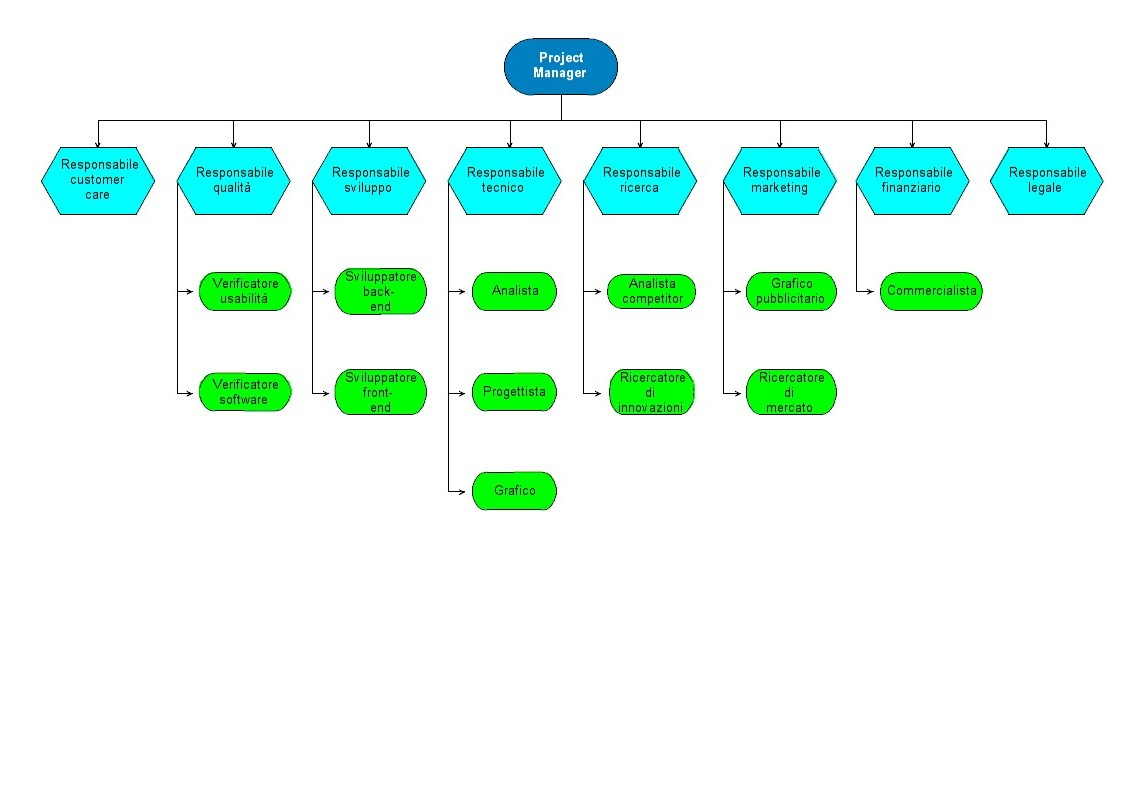
\includegraphics[scale=0.5]{img/Progetto2.jpg}
\caption{Diagramma OBS}
\label{fig:Diagramma OBS}
\end{figure}

\subsubsection{Project manager}
Responsabile ultimo del completamento del progetto, i suoi obblighi comprendono:
\begin{itemize}
\item realizzazione del progetto nel rispetto dei requisiti funzionali, di qualit\`{a} e dei
vincoli imposti;
\item rispetto dei tempi di consegna e dei costi preventivati;
\item rispetto dei margini di profitto preventivati.
Per assicurarsi di far fronte ai suoi obblighi, il PM pianifica tutte le fasi del progetto
coordinando le risorse per assicurare il conseguimento degli obbiettivi, anche in caso di
circostanze inaspettate.
\end{itemize}

\subsubsection{Responsabile costumer care}
Il RCC deve:
\begin{itemize}
\item scegliere le modalit\`{a} con cui gli utenti possono comunicare all\textquoteright{}azienda;
\item scegliere i servizi a cui appoggiarsi per gestire il rapporto con i clienti;
\item intrattenere rapporti diretti con i clienti pi\`{u} importanti, eventualmente con il
supporto del PM;
\item stendere rapporti mensili (da consegnare al PM) inerenti le maggiori problematiche
riscontrate dai clienti o con i mezzi di comunicazione e i servizi adottati.
\end{itemize}

\subsubsection{Responsabile qualit\`{a}}
Il RQ ha il compito di definire gli standard di qualit\`{a} da rispettare per ogni singolo processo
svolto dall\textquoteright{}azienda e di promuovere il miglioramento dei processi in corso di sviluppo.
Si attiene strettamente alle normative in materia di qualit\`{a} (ISO 9000/9001/9004
e ISO 9126 relativamente alla qualit\`{a} del software) e, a seguito dell\textquoteright{} analisi dei singoli
processi, promuove azioni di miglioramento, sia attraverso comunicazioni interne all\textquoteright{}azienda,
che attraverso formazione specifica degli addetti. Il miglioramento continuo
della qualit\`{a} aziendale, seguendo le linee guida del CMMI\footnote{Capability Maturity Model Integration - \url{http://it.wikipedia.org/wiki/Capability\_Maturity\_Model}}, garantisce all\textquoteright{}azienda un
miglioramento dell\textquoteright{}efficienza ed una maggiore soddisfazione dei clienti. Per quanto riguarda
il prodotto software sviluppato, il RQ deve inoltre comunicare al PM i verbali
ottenuti dai suoi sottoposti e proporre attivit\`{a} mirate all\textquoteright{}incremento della qualit\`{a}.

\subsubsection{Verificatore usabilit\`{a}}
L\textquoteright{}azienda crede fermamente che un prodotto altamente usabile (vedi ISO 9241) sia
sinonimo di qualit\`{a} e sia in parte garanzia di successo. Per questo motivo, contemporaneamente
alla verifica di accessibilit\`{a} del prodotto, il verificatore valuter\`{a} eventuali
migliorie sul piano dell\textquoteright{}usabilit\`{a} e rediger\`{a} un verbale per il RQ esponendo le eventuali problematiche riscontrate e le possibili soluzioni.

\subsubsection{Verificatore software}
Tra le varie fasi che compongono la creazione di un prodotto software, c\textquoteright{}\`{e} il testing.
Questa operazione viene svolta dagli sviluppatori (SF e SB) e punta all\textquoteright{}eliminazione del
maggior numero di bug possibili. Una fase altrettanto importante \`{e} quella della verifica
e della validazione del software (vedi IEEE 1012), in questo caso il VS deve controllare
che quanto prodotto rispetti i requisiti espressi nel documento di Analisi dei Requisiti
redatto dall\textquoteright{}analista e sia effettivamente quanto richiesto. Al termine di ogni sessione di verifica il VS rediger\`{a} un verbale per il RQ.

\subsubsection{Responsabile tecnico}
Il RT coordina ogni fase dello sviluppo dei prodotti software dell\textquoteright{}azienda ed \`{e} il responsabile
dello stato di avanzamento dei prodotti nel rispetto delle scadenze temporali e
dei costi. Ha una competenza tecnica molto vasta e deve potersi
relazionare con i suoi subordinati su ogni aspetto dello sviluppo.\\
Una volta ricevuto l\textquoteright{}incarico dal PM:
\begin{enumerate}
\item assegna all\textquoteright{}analista il compito di formalizzare quanto dev\textquoteright{}essere prodotto;
\item al termine della fase di analisi, incarica:
\begin{itemize}
\item il Progettista di delineare l\textquoteright{}architettura di dettaglio;
\item il Grafico di stendere le bozze delle interfacce utente.
\end{itemize}
\item durante la fase di progettazione, il RT controlla che l\textquoteright{}architettura software rispetti
le metriche software concordate e propone al progettista eventuali modifiche. Nel
caso fosse necessario (utilizzo di un nuovo linguaggio/framework), predispone corsi
di aggiornamento o di formazione per gli sviluppatori;
\item al termine della fase di progettazione, consegna quanto prodotto al RS;
\item coordina le operazioni di manutenzione successive al rilascio.
\end{enumerate}

\subsubsection{Analista}
L\textquoteright{}analista ha il compito di formalizzare quanto emerso dalle discussioni con il PM e
dalla lettura della documentazione di presentazione del progetto. Redige lo "Studio di Fattibilit\`{a}", nel quale si indica se il progetto \`{e} fattibile e quali sono le aree critiche ed il documento di Analisi dei Requisiti nel quale, con l\textquoteright{}ausilio di diagrammi dei casi d\textquoteright{}uso e di altri formalismi(vedi INCOSE\footnote{International Council on Systems Engineering - \url{http://www.incose.org/}}), viene riportato cosa sar\`{a} sviluppato. Al termine della fase di analisi l\textquoteright{}analista consegner\`{a} entrambi i documenti al RT.

\subsubsection{Progettista}
La fase di progettazione ha inizio con la delibera, da parte del PM, di quanto prodotto
dall\textquoteright{}analista e con la conseguente assegnazione dell\textquoteright{}incarico al Progettista. Una volta
studiata l\textquoteright{}Analisi dei Requisiti, il progettista redige dapprima il documento di "Specifica
Tecnica", nel quale viene proposta una soluzione ad alto livello del problema focalizzandosi
maggiormente sulle funzionalit\`{a}, piuttosto che sulla loro implementazione, e successivamente
il documento di "Definizione di Prodotto" nel quale si propone una soluzione concreta e
dettagliata al problema posto. In entrambi i documenti il progettista far\`{a} ampio uso di
diagrammi e schemi per rendere il pi\`{u} chiara possibile qualsiasi scelta implementativa.
Al termine della fasi di progettazione i documenti prodotti sono consegnati al RT.

\subsubsection{Grafico}
Il grafico viene incaricato dal RT di creare le bozze per ogni interfaccia utente presente
nel progetto. Il lavoro inizia con la lettura dell\textquoteright{}"Analisi dei Requisiti" e, in particolare,
con la sezione relativa ai casi d\textquoteright{}uso che indicano, tra l\textquoteright{}altro, quante possibili bozze sono
necessarie. Una volta create, le bozze vengono consegnate al PM che le valuta con
l\textquoteright{}ausilio del team del RQ e, se necessario, con il RDM.

\subsubsection{Responsabile sviluppo}
Il RS coordina ogni fase dello sviluppo dei prodotti software dell\textquoteright{}azienda ed \`{e} il responsabile
dello stato di avanzamento dei prodotti nel rispetto delle scadenze temporali e
dei costi. Ha una competenza tecnica molto vasta assimilata e deve potersi
relazionare con i suoi subordinati su ogni aspetto dello sviluppo. Una volta ricevuto
l\textquoteright{}incarico dal RT in accordo con il PM:
\begin{itemize}
\item suddivide gli incarichi di lavoro tra SF e SB in base a quanto fornito dal RT;
\item durante la fasi di sviluppo, segue attentamente i report relativi ai test effettuati e
controlla lo stato di avanzamento del prodotto in relazione alle scadenze prefissate;
\item supervisiona le fasi di alpha e beta testing ed i successivi test di collaudo precedenti
il rilascio.
\end{itemize}

\subsubsection{Sviluppatore front-end}
Lo SF viene incaricato dal RS di realizzare e successivamente manutenere tutte le parti
software con cui interagisce l\textquoteright{}utente, oltre ai documenti tecnici prodotti dal Progettista
gli vengono consegnate anche le bozze create dal Grafico.

\subsubsection{Sviluppatore back-end}
Lo SB viene incaricato dal RS di realizzare e successivamente manutenere tutte le parti
software che elaborano dati e non sono a diretto contatto con l\textquoteright{}utente, per svolgere il
suo compito necessita solo dei documenti tecnici prodotti dal Progettista.

\subsubsection{Responsabile ricerca}
Il mercato attuale \`{e} in continua evoluzione ed anche potendo contare su un prodotto
di successo, bisogna essere in grado di migliorarlo continuamente per poter rimanere al
passo rispetto alla concorrenza. Il RR quindi coordina il suo team per:
\begin{itemize}
\item rimanere al passo con i competitor, analizzando le funzionalit\`{a} da loro
implementate e capendo quali di esse potrebbero dare un valore aggiunto al
progetto;
\item creare un gap rispetto ai competitor, cercando soluzioni innovative non ancora
presenti sul mercato e che facciano evolvere positivamente il progetto.
\end{itemize}

\subsubsection{Analista competitor}
L\textquoteright{}AC deve scandagliare tutti i "rivali" del prodotto che si sta sviluppando e cercare
di capire quali delle soluzioni da loro implementate possano dare un tangibile valore
aggiunto al progetto. A ricerca completata l\textquoteright{}AC produrr\`{a} una documentazione di quanto
trovato e la consegner\`{a} per valutazione al RR.

\subsubsection{Ricercatore di innovazioni}
Il RI basandosi su quanto reso disponibile dal prodotto e su eventuali trend di mercato
in settori affini, cerca di trovare novit\`{a} da poter implementare nel prodotto al fine di
aumentare: le funzionalit\`{a} offerte, la soddisfazione dell\textquoteright{}utente, il bacino di utenza e di
estendere eventualmente il target del prodotto. Al termine del processo il RI produrr\`{a}
una documentazione che sar\`{a} consegnata per valutazione al RR.

\subsubsection{Responsabile marketing}
Il RM ha l\textquoteright{}onere di posizionare i prodotti nel mercato di riferimento e di renderli profittevoli.
Per adempiere al suo compito analizza il mercato individuando cos\`{i} le opportunit\`{a}
di business e progetta ed attua le strategie di marketing pi\`{u} efficaci per l\textquoteright{}incremento
dei profitti e per l\textquoteright{}affermazione del brand.

\subsubsection{Grafico Pubblicitario}
Per far conoscere l\textquoteright{}azienda ai possibili utilizzatori e per stimolare l\textquoteright{}adozione dei prodotti
proposti \`{e} indispensabile avere campagne pubblicitarie efficaci. Il GP, sotto la
supervisione del RM, crea le pubblicit\`{a} dell\textquoteright{}azienda.

\subsubsection{Ricercatore di mercato}
Il RDM ha competenze statistiche specifiche nella creazione di sondaggi e nell\textquoteright{}analisi
dei dati ottenuti; ha lo scopo di comprendere qual \`{e} l\textquoteright{}opinione delle persone relativamente
all\textquoteright{}azienda e ai prodotti da essa sviluppati e quali sono, in generale, gli aspetti
migliorabili. Si occupa, quindi, di redigere sondaggi ai fini di comprendere:
\begin{itemize}
\item qual \`{e} il target di riferimento;
\item quanto gli utenti conoscono i prodotti sviluppati dall\textquoteright{}azienda;
\item il livello di qualit\`{a} e seriet\`{a} che gli utenti attribuiscono all\textquoteright{}azienda e ai suoi
prodotti;
\item eventuali aspetti negativi riscontrati o miglioramenti proposti.
\end{itemize}

\subsubsection{Responsabile finanziario}
Il RF ha il compito di monitorare il flusso di cassa dell\textquoteright{}azienda e di individuare eventuali
problematiche ben prima che si verifichino. Si avvale di un Commercialista per le
operazioni contabili e di un BF per massimizzare le rendite dell\textquoteright{}azienda.

\subsubsection{Commercialista}
Il Commercialista \`{e} incaricato dall\textquoteright{}azienda di mantenerne la contabilit\`{a}, di effettuare i
versamenti delle tasse e di verificare e legittimarne le operazioni economiche.

\subsubsection{Responsabile legale}
Il RL viene contattato dall\textquoteright{}azienda quando:
\begin{itemize}
\item si vuole garantire che i software sviluppati rispettino le normative vigenti, nello
specifico quelle relative alla privacy;
\item si vogliono archiviare particolari brevetti o si vuole garantire il copyright di un
prodotto;
\item nascono dispute legali tra terzi e l\textquoteright{}azienda;
\item si sviluppano trattative economiche delle quali non \`{e} del tutto chiara la legittimit\`{a}.
\end{itemize}


\subsection{Resource Breakdown Structure}
La Resource Breakdown Structure, d'ora in poi RBS, identifica ed esplicita tutte le
risorse necessarie alla realizzazione del progetto. Queste vengono classificate a seconda della
loro categoria e tipologia. Con il termine risorsa si intende specificare ogni singola
componente fra tutto quello che risulta essere utile e necessario per lo svolgimento e la
buona riuscita del progetto: le risorse umane, i materiali, le attrezzature ed il tempo;
ovvero componenti a cui sia possibile attribuire un costo in denaro per il loro utilizzo. La
RBS si dimostra un ottimo strumento di supporto alla pianificazione in quanto consente
di ottimizzare l'impiego di ogni singola risorsa necessaria, inoltre la RBS risulta essere fortemente
legata alla stima dei costi in quanto questi vengono generati in base all'impiego delle
risorse descritte.

\begin{figure}[H]
\centering % per centrare l'immagine (opzionale)
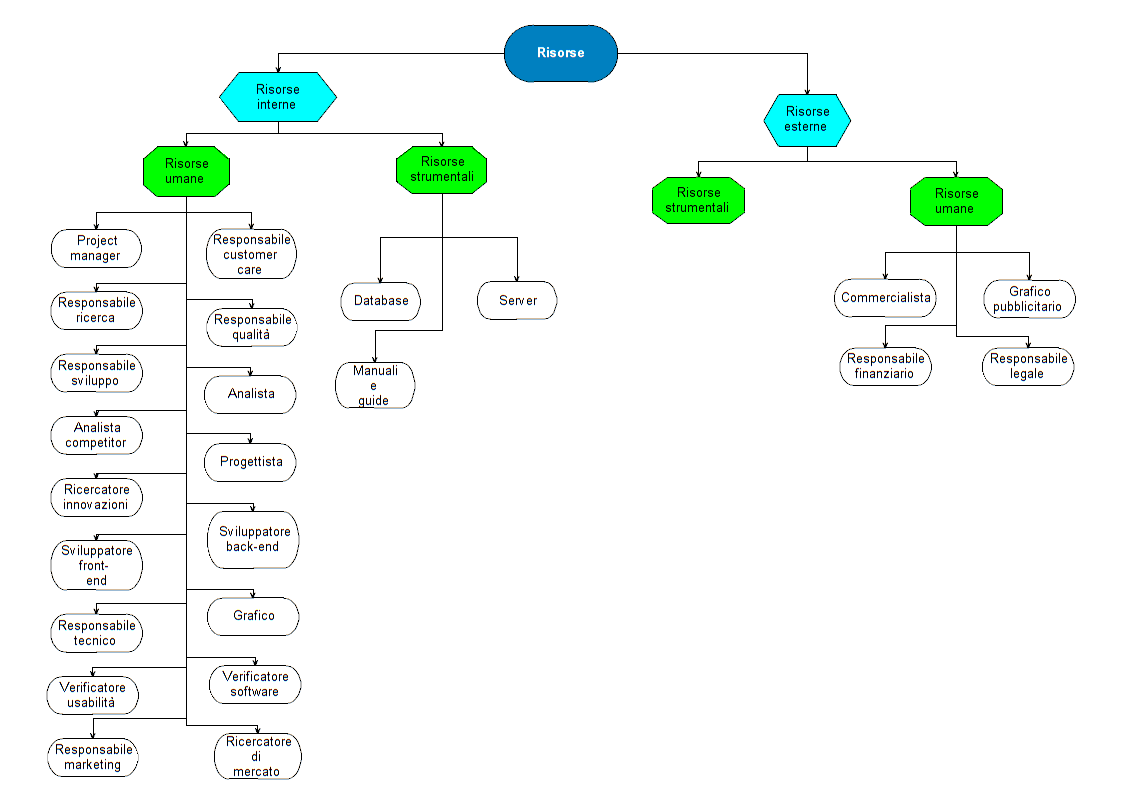
\includegraphics[scale=0.5]{img/Risorse_rbs.png}
\caption{Diagramma RBS}
\label{fig:Diagramma RBS}
\end{figure}


\subsection{Pianificazione temporale}
\subsubsection{Diagramma di Gantt}

I diagrammi di Gantt sono una rappresentazione su scala temporale dell'evoluzione del
progetto. Sono composti da varie barre orizzontali ognuna delle quali rappresenta una
attivit\'a che viene collocata sulla scala temporale in rappresentanza dell'attivi\'a stessa.
I diagrammi di Gantt hanno lo scopo di:
\begin{itemize}
\item definire cosa fare in una certa quantit\'a di tempo;
\item definire un riferimento per il controllo dell'avanzamento;
\item  definire degli eventi chiave dette milestones (fine di una fase, consegna).
\end{itemize}
Un diagramma di Gantt consente quindi la rappresentazione grafica di un calendario di
attivit\'a facilitando la pianificazione, il coordinamento e il tracciamento delle specifiche
attivit\'a dando una illustrazione dello stato di avanzamento del progetto. Per costruire
un diagramma di Gantt bisogna:
\begin{itemize}
\item  determinare le attivit\'a necessarie per concludere il progetto;
\item  stabilire il limite temporale del progetto;
\item  disegnare sul grafico il limite temporale stimato per ciascuna attivit\'a;
\item  verificare la presenza di discrepanze tra il tempo stimato e quello effettivamente
utilizzato.
\end{itemize}
Tramite i diagrammi di Gantt si identifica il percorso critico: alcune attivit\'a possono
partire solo dopo che altre sono finite, ognuna di queste attivit\'a viene detta critica e la
loro unione forma il percorso critico. \'E molto importante che le attivit\'a critiche non
subiscano slittamenti poich\'e questi si ripercuoterebbero, a cascata, su tutte le attivit\'a
critiche in attesa.

\subsubsection{Microsoft Project 2013}
Per la gestione e la pianificazione del progetto si \'e scelto di usare Project2013 essendo
un software dedicato al Project Management. Project2013 
crea automaticamente i diagrammi di Gantt una volta inserite le singole attivit\'a. Il software permette, inoltre, di modificare
le relazioni tra le attivit\'a e le date di inizio e fine nel caso le previsioni fatte non si
verifichino veritiere, o per l'insorgenza di problemi inaspettati. Questa funzionalit\'a
permette di mantenere il piano di progetto aggiornato con gli ultimi avvenimenti e d\'a
un idea del ritardo (o anticipo) acquisiti.

\subsubsection{Visione Globale del Progetto}
Viene presentata in questa sezione la visione generale del piano di progetto in modo da
dare una visione delle dipendenze tra le varie fasi, consentendo di comprendere:
\begin{itemize}
\item l'evoluzione temporale dell'intero progetto;
\item quanto pesa percentualmente ogni fase sia in senso economico che di tempo;
\item l'impiego delle varie risorse.
\end{itemize}
Di seguito sono presentate le immagini dei work package, ossia delle macro-attivit\'a in cui
\'e stato suddiviso il progetto, il diagramma di Gantt dell'intero progetto.
Il progetto risulta quindi avere un costo di \euro{}, a cui si dovranno andare a
sommare i costi di mantenimento e hosting del servizio.

\begin{figure}[H]
\begin{center}
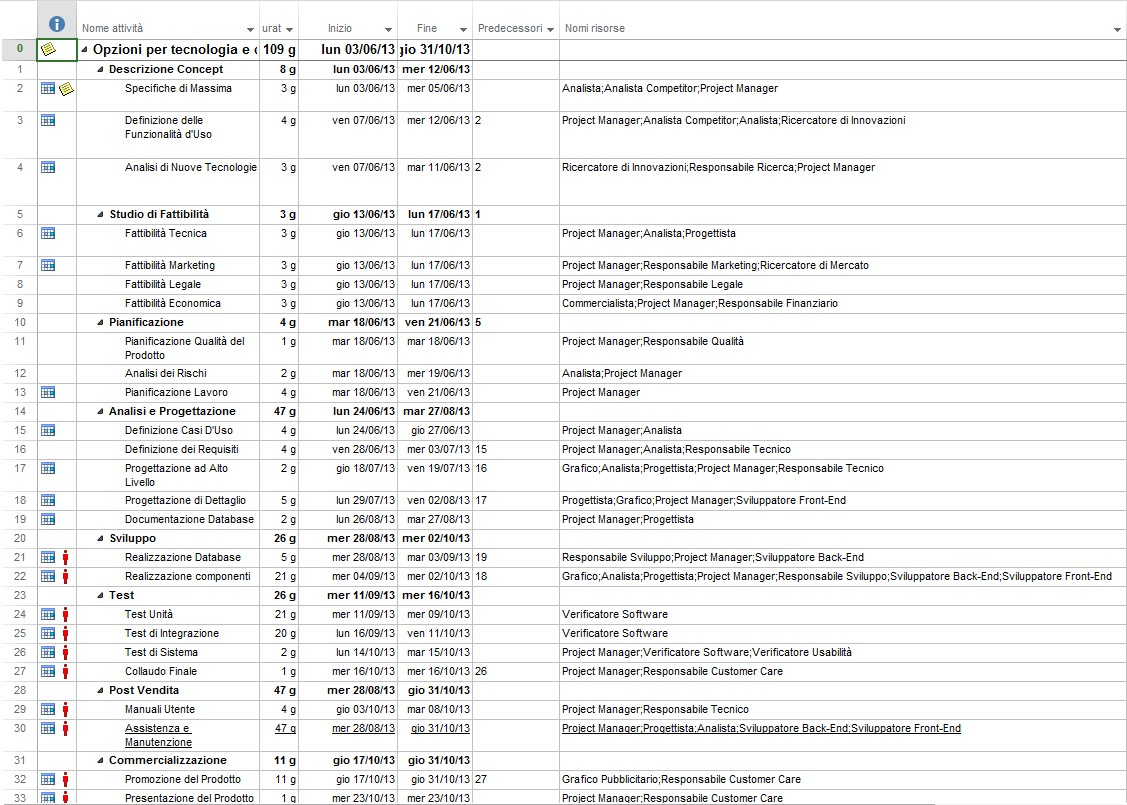
\includegraphics[width=1\textwidth]{img/Attivita.jpg}
\caption{Diagramma  Attivit\'a}
\label{fig:Diagramma Attivit\'a}
\end{center}
\end{figure}
\begin{figure}[H]
\begin{center}
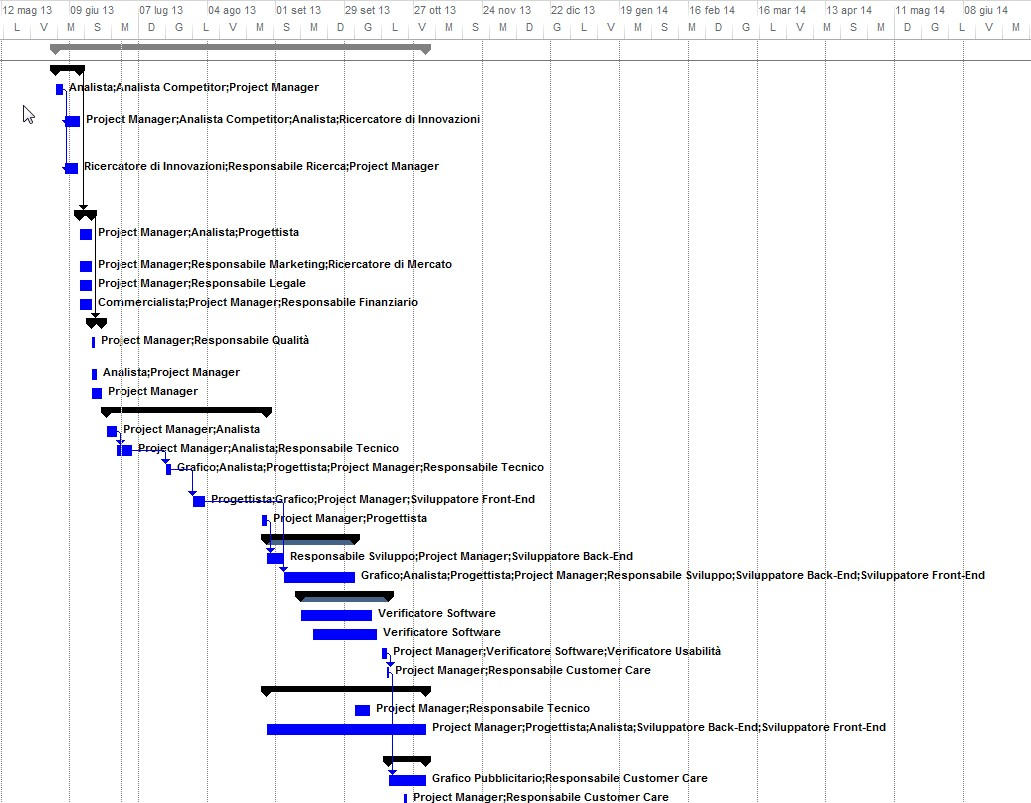
\includegraphics[width=1\textwidth]{img/Gantt.jpg}
\caption{Gantt Progetto}
\label{fig:Gantt Progetto}
\end{center}
\end{figure}
\newpage
\subsubsection{Gantt Milestone}

\begin{figure}[H]
\begin{center}
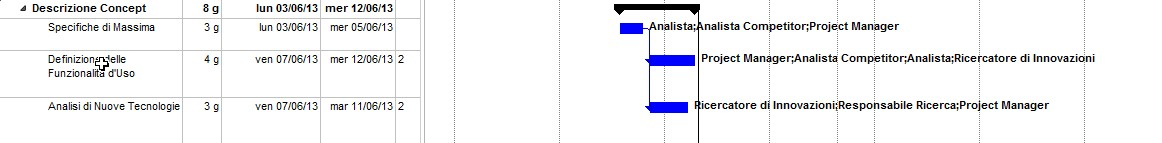
\includegraphics[width=1\textwidth]{img/G-A Concept.jpg}
\caption{Gantt Definizione Concept}
\label{fig:Gantt Definizione Concept}
\end{center}
\end{figure}

\begin{figure}[H]
\begin{center}
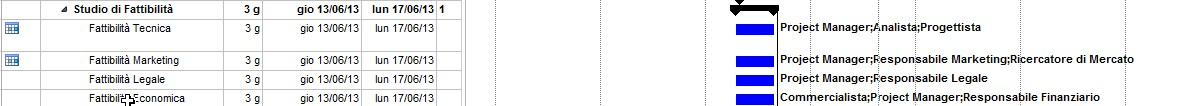
\includegraphics[width=1\textwidth]{img/G-A Fattibilita.jpg}
\caption{Gantt Studio di Fattibilit\'a}
\label{fig:Gantt Studio di Fattibilit\'a}
\end{center}
\end{figure}

\begin{figure}[H]
\begin{center}
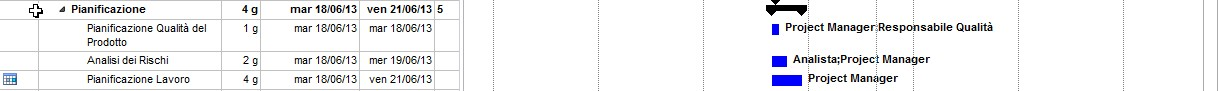
\includegraphics[width=1\textwidth]{img/G-A Pianificazione.jpg}
\caption{Gantt Pianificazione}
\label{fig:Gantt Pianificazione}
\end{center}
\end{figure}

\begin{figure}[H]
\begin{center}
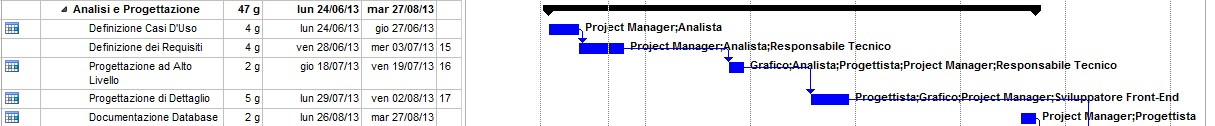
\includegraphics[width=1\textwidth]{img/G-A Analisi.jpg}
\caption{Gantt Analisi e Progettazione}
\label{fig:Gantt Analisi e Progettazione}
\end{center}
\end{figure}

\begin{figure}[H]
\begin{center}
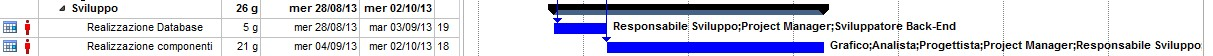
\includegraphics[width=1\textwidth]{img/G-A Sviluppo.jpg}
\caption{Gantt Sviluppo}
\label{fig:Gantt Sviluppo}
\end{center}
\end{figure}

\begin{figure}[H]
\begin{center}
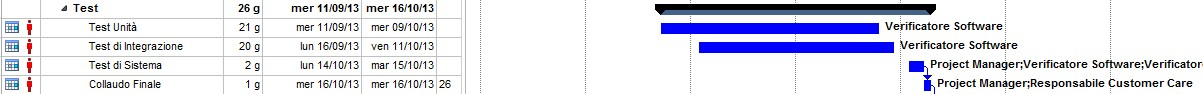
\includegraphics[width=1\textwidth]{img/G-A Test.jpg}
\caption{Gantt Test}
\label{fig:Gantt Test}
\end{center}
\end{figure}

\begin{figure}[H]
\begin{center}
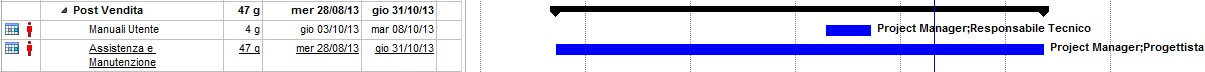
\includegraphics[width=1\textwidth]{img/G-A Vendita.jpg}
\caption{Gantt Vendita}
\label{fig:Gantt Vendita}
\end{center}
\end{figure}

\begin{figure}[H]
\begin{center}
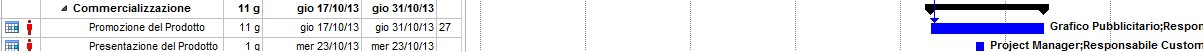
\includegraphics[width=1\textwidth]{img/G-A Commercializzazione.jpg}
\caption{Gantt Commercializzazione}
\label{fig:Gantt Commercializzazione}
\end{center}
\end{figure}
\newpage

\section{Qualità}
\paragraph*{Qualit\`{a} processi}

Il team prevede nella gestione di questo progetto degli obiettivi di qualit\`{a} affini non solo al progetto stesso, ma anche al team inteso come organizzazione.\\
Occorrer\`{a} quindi documentare ci\`{o} che sono le norme, le convenzioni e le procedure fissandole in base alle best practices acquisite dal team dallo sviluppo di progetti precedenti. Tutte le informazioni utili allo svolgimento delle attivit\`{a} dovranno essere organizzate e aggiornate, applicando cos\`{i} la logica del ciclo PDCA.

\begin{figure}[H]
\begin{center}
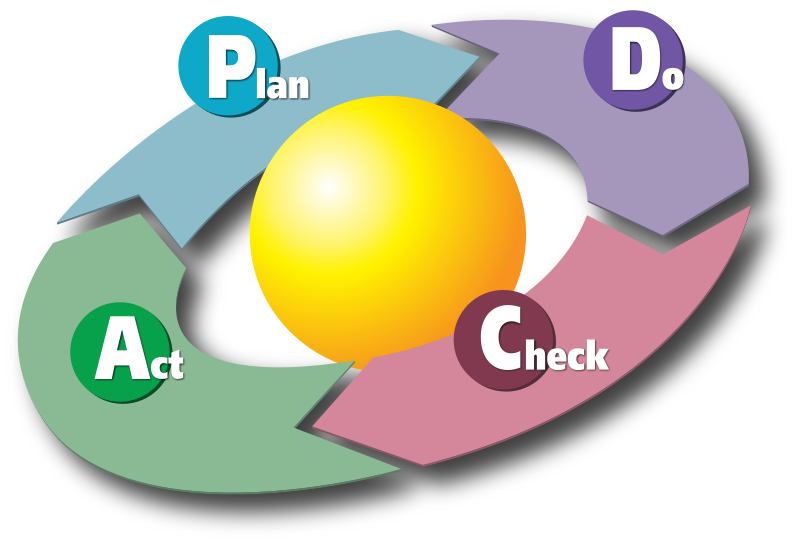
\includegraphics[width=0.60\textwidth]{img/pdca.png}
\caption{Ciclo PDCA}
\label{fig:PDCA}
\end{center}
\end{figure}

La qualit\`{a} dovr\`{a} rigurdare quindi, in primis, l\textquoteright{}organizzazione del lavoro al fine che esso sia il pi\`{u} possibile regolato e ordinato, poi potr\`{a} anche riflettersi nel progetto.

\paragraph*{Qualit\`{a} software}

Gli obiettivi di qualit\`{a} andranno distinti in ogni fase del ciclo di vita del software. Qui verranno elencati i principali obiettivi nelle fasi critiche, cio\`{e} le milestones del progetto.

\subparagraph{Analisi}
\begin{itemize}
\item Fissare incontri con i possibili clienti interrogandoli sulle funzionalit\`{a} desiderabili del prodotto;
\item Raccogliere pi\`{u} feed-back possibile, quindi tenere aggiornati i requisiti al fine di fornire un prodotto, il pi\`{u} possibile secondo le aspettative dei clienti.
\end{itemize}
\subparagraph{Progettazione}
\begin{itemize}
\item L\textquoteright{}architettura dovr\`{a}, ove possibile, integrare compenenti gi\`{a} realizzate e testate al fine di riutilizzarle senza realizzarle poi da zero;
\item L\textquoteright{}architettura dovr\`{a} implementare solo design patterns conosciuti e dimostati;
\item L\textquoteright{}architettura dovr\`{a} limitare il numero di dipendenze tra le componenti ed evitare le dipendenze cicliche;
\item L\textquoteright{}architettura dovr\`{a} utilizzare componenti che prevedono l\textquoteright{}utilizzo di classi che implementano metodi il cui codice non superi le 50 righe;
\item L\textquoteright{}architettura dovr\`{a} essere sottoposta a revisione da parte di entit\`{a} non direttamente coinvolte.
\end{itemize}
\subparagraph{Sviluppo}
\begin{itemize}
\item Il codice dell\textquoteright{}applicativo dovr\`{a} essere commentato nei punti critici;
\item Il codice dell\textquoteright{}applicativo dovr\`{a} avere una bassa complessit\`{a} ciclomatica\footnote{\url{http://it.wikipedia.org/wiki/Complessit\%C3\%A0\_ciclomatica}};
\item La compilazione del codice non dovr\`{a} fornire né errori né warnings\footnote{Gli avvisi sono messaggi di diagnostica, inviati dal compilatore, che riportano costruzioni che non sono intrinsecamente erronee, ma che sono rischiose o suggeriscono che potrebbe esserci un errore.}.
\end{itemize}
\newpage


\section{Gestione dei rischi}
\subsection{Indisposizione del personale} 
\begin{description}
\item[Descrizione:]c'è la possibilità che uno, o più membri del gruppo di lavoro, non possa prendere parte attivamente al progetto per un periodo di tempo variabile causa malattia o impegni personali importanti. Ciò può comportare dei rallentamenti, fino al possibile mancato rispetto dei termini di rilascio previsti.

\item[Soluzione:] In tale circostanza, il gruppo di lavoro sarà considerato in stato d'emergenza. Il responsabile del gruppo o, in mancanza, il PM, ha l'onere di decidere se:
\begin{itemize}
\item l'assente può continuare il proprio lavoro temporaneamente tramite telelavoro;
\item è possibile ridistribuire (tutto o in parte) il lavoro tra i restanti membri del gruppo;
\item si rende necessaria l'assunzione temporanea di nuovo personale;
\item tale assenza comporterà o meno un ritardo del progetto.
\end{itemize}
Se l'indisponibilità tuttavia permane, senza motivi validi, il responsabile dovrà dapprima cercare di risolvere il problema con l'interessato e, in ultima istanza, contattare gli organi sindacali competenti.
\item[Impatto:] 4, se ciò colpisce più membri contemporaneamente, l'impatto può essere gravoso e portare a rallentamenti significativi.
\item[Probabilità:] 3.
\item[Controllo:] Qui sono fondamentali le figure del responsabile e del PM che dovranno monitorare l'avanzamento del progetto ed agire tempestivamente in caso di assenze o ritardi per non causare rallentamenti nello sviluppo del prodotto, è inoltre importante comunicare repentinamente eventuali indisponibilità agli altri membri del gruppo, soprattutto se programmabili, per permettere al responsabile di redistribuire il carico di lavoro correttamente ed in modo efficiente. 
\end{description}

\subsection{Fallimento del progetto}
\begin{description}
\item[Descrizione:] Il prodotto che l'azienda vuole sviluppare è presente sul mercato, ma i numerosi rivali (competitor) che propongono questo tipo di prodotto si sono cimentati solamente nello sviluppo dell'applicativo per piattaforma Microsoft senza dare importanza a altre piattaforme come Linux.
Il rischio è quindi che i competitor aggiornino i loro prodotti includendo anche le
funzionalità da noi proposte(sviluppo per più piattaforme) e, forti di una base di utenti molto ampia, non permettano ulteriori sviluppi del progetto decretandone una fine prematura. La sola presenza nel mercato di altri competitor con un'ampia base di utenza, pone il progetto a rischio di fallimento.
\item[Soluzione:] Per cercare di minimizzare il più possibile tale rischio si adotteranno le
seguenti procedure:
\begin{itemize}
\item nelle fasi precedenti all'analisi e alla progettazione del prodotto sarà posta
massima cura nel pregi e difetti delle soluzioni adottate dai competitor, oltre ad evidenziarne eventuali parti
migliorabili. Sarà posta anche particolare cura nel capire quali sono le mind maps degli utenti che utilizzano prodotti affini a quello sviluppato e si cercherà di replicarle nel prodotto finito. Tale strategia permette all'azienda di partire avvantaggiata nello sviluppo del prodotto, cercando di replicare il feeling che l'utente ha sviluppato con prodotti affini e cercando di migliorare i difetti comuni.
\item nelle fasi immediatamente precedenti al rilascio sarà fatta una campagna
pubblicitaria massiva e che punti a far crescere l'interesse verso il nostro prodotto.
\item nelle fasi successive al rilascio la campagna pubblicitaria dovrà rendere chiaro
in cosa il prodotto si distingue rispetto ai concorrenti.
\item l'azienda dovrà porre particolare cura al rapporto con gli utenti e dovrà
proporre soluzioni o migliorie tempestive basandosi sui possibili consigli da parte del pubblico.
\item l'azienda in generale dovrà mettere in atto quanto descritto nella sezione Pubblicità  del documento
\end{itemize}
\item[Impatto:] 5, la mancata adozione del nostro prodotto da parte degli utenti porterebbe
al fallimento stesso del progetto.
\item[Probabilità:] 3, il numero di competitor non è molto elevato ed il rischio che loro adattino
il loro prodotto includendo le novità da noi proposte è sostanziale. 
\item[Controllo:] Il PM deve monitorare attentamente gli indicatori di utilizzo del prodotto
e valutare settimanalmente quali azioni compiere per incrementarli.
\end{description}

\subsection{Difficoltà nel pianificare correttamente i tempi di sviluppo}
\begin{description}
\item[Descrizione:] C'è il forte rischio di effettuare una stima errata in materia di ore/persona necessarie allo svolgimento dell'intero progetto e della loro allocazione alle rispettive figure professionali in gioco. Le ore schedulate infatti potrebbero essere
insufficienti o allocate in ruoli in cui ne sono sufficienti un numero minore. Il mancato utilizzo
di un modello di sviluppo lungimirante, potrebbe portare a una serie di
iterazioni dannose per il progetto. Il rischio, quindi, e quello di non rispettare una
delle milestone previste per il progetto e di perdere ulteriore strada rispetto alla concorrenza.
\item[Soluzione:] Nella pianificazione delle milestone si è tenuto conto di questo rischio e si è
cercato di pensare a tutti i possibili fattori che potrebbero porre problemi al riguardo.
\item[Impatto:] 4, forti errori potrebbero portare seri problemi al gruppo e alla realizzazione del progetto.
\item[Probabilià:] 5, problematica praticamente inevitabile.
\item[Controllo:] Fondamentale è il ruolo del PM e degli altri responsabili, che devono sempre
tenere monitorato l'avanzamento del proprio lavoro e reindirizzare le risorse
dove maggiormente necessarie al fine di rispettare le milestone previste, con gli
obiettivi di qualità posti.
\end{description}

\subsection{Analisi dei requisiti non corretta}
\begin{description}
\item[Descrizione:] Fondamentale per il successo del progetto è un'analisi dei requisiti di
qualità ed uno studio molto approfondito del bisogno degli utenti target e delle
caratteristiche positive e negative dei competitor analizzati. Un errore in questa fase
del progetto sarebbe identificato solamente nei primi test pubblici del prodotto,
il che significherebbe dover riprendere per mano l'intero processo di sviluppo con
significative perdite di tempo e risorse.
\item[Soluzione:] La ripartizione oraria terrà conto della necessità di assegnare un numero
sostanzioso di ore al processo di analisi e sarà utilizzato, ove necessario,
personale esterno altamente qualificato al fine di garantire una buona riuscita di
questo processo così critico. 
\item[Impatto:] 5, un processo di analisi completato frettolosamente potrebbe portare a gravi rallentamenti ed anche al fallimento del progetto.
\item[Probabilità:] 2, nonostante le misure intraprese per evitare questo problema, saranno sicuramente possibili delle problematiche relative ai requisiti.
\item[Controllo:] Il PM  accertarsi che quanto prodotto durante il processo di analisi sia in linea con la visione aziendale; tuttavia sarà solo nelle fasi di test da parte degli utenti che si potranno delineare eventuali problematiche.
\end{description}

\subsection{Cause legali}
\begin{description}
\item[Descrizione:] Vista la tipologia di prodotto sviluppato e vista la grande quantità di
dati personali memorizzati, è possibile che un competitor o un gruppo di utenti, decidano di fare causa all'azienda.
\item[Soluzione:] Per evitare che i competitor agiscano legalmente contro l'azienda bisogna porre massima cura nell'accertarsi che le idee o i software utilizzati non vengano usati in maniera illegale e che i brevetti di terzi siano rispettati. Per
quanto riguarda le azioni legali intraprese dagli utenti si possono evidenziare 2
motivazioni:
\begin{itemize}
\item privacy: in questo caso basterà informare preventivamente gli utenti di come
i loro dati verranno salvati all'interno del database.
\item  altro: un utente potrebbe far causa all'azienda per le motivazioni più svariate
(es.: tematiche affrontate in certi progetti, commenti fatti dai dipendenti
dell'azienda, ecc); in questo caso sarà il RL a valutare il miglior modo di
gestire la situazione.
\end{itemize}
\item[Impatto:] 5, una causa legale può protrarsi per per molto tempo e portare ad uno spreco di finanze
dell'azienda mettendo a rischio il progetto stesso.
\item[Probabilità:] 2, bisognerà stare molto attenti essendo una problematica spesso presente.
\item[Controllo:] Il RL dovrà definire attentamente i contratti e tutta la documentazione
legale. Il PM dovrà chiamarlo prontamente in causa alle prime avvisaglie di
problematiche legali, in modo da poterle risolvere nel minor tempo possibile.
\end{description}


\newpage


\end{document}
